\subsection{AoA aux}


Analisando a defasagem de sinal \ac{RF} em um conjunto de antenas, é possível estimar seu \acf{AoA}, essa técnica pode ser utilizada para determinar a direção do emissor em relação à matriz de antenas utilizada.
Baseando-se em dados como a distância entre as antenas, o comprimento de onda $\lambda$ do sinal e a velocidade da luz no meio, usualmente tomada como $c = \SI{299792458,6 \pm 0,3}{\metre\per\second}$ no ar \cite{jennings1987continuity, bensky2016wireless, horst2021localization}.
A \autoref{eq:wavelength} apresenta a relação do comprimento de onda $\lambda$ com a frequência $f$, a frequência angular $\omega$ e a velocidade da luz $c$.

\begin{equation} \label{eq:wavelength} % Comprimento de onda
    \lambda = \frac{c}{f} = \frac{2\pi \cdot c}{\omega}
\end{equation}

Se um emissor de sinal estiver distante o suficiente, é possível considerar que a frente de onda tem um comportamento planar, essa característica simplifica as operações envolvidas.
A distância de Fraunhofer ($d_F$) é a mínima para essa condição, que define o início da região de \textit{far-field}, conforme apresentado na \autoref{eq:fraunhofer}, onde $D$ é a maior dimensão da antena \cite{balanis2016antenna}.
Tomando $D = 2  \lambda$, para uma antena de dipolo, obtém-se $d_F = 8 \lambda$.
A \autoref{fig:plana_0} ilustra o comportamento planar de uma frente de onda, com destaque na distância $d_F$.

\begin{equation} \label{eq:fraunhofer}
    d_F = \frac{2 \cdot D^2}{\lambda} \quad \Rightarrow \quad d_F = \frac{2 \cdot \left(2 \cdot \lambda \right)^2}{\lambda} = 8 \lambda
\end{equation}

\begin{figure}[htpb]
    \centering
    \caption{Característica de frente de onda a cada $\lambda$ a partir da antena emissora.}
        % \resizebox{\textwidth}{!}{%
    \begin{circuitikz}[american, voltage shift=0.5, line width=0.5]

        \def\wavelength{0.5}
        \def\d{0.5*\wavelength}

        \def\closeRange{1}
        \def\farRange{\closeRange+30}

        \coordinate (O) at (0,0);
        \coordinate (antenna) at (-\closeRange,0);
        % \draw [help lines, dashed] (-5,-3) grid (5,3); % desenha grid
        % \draw [red] (O) node[draw,cross out] {}; % marca pont(0,0)

        \draw[thick]
            (antenna) node[dinantenna, scale=0.75]{}
        ;

        % \draw (\closeRange-0.5,-4) rectangle (\farRange+0.1,4);
        \clip (-0.75,-1.5) rectangle (12.1,1.5);
        \foreach \x [evaluate={\z=int((\x+\closeRange));}] in {0,...,30} {
            \draw [gray, thin, opacity=0.5] (antenna) circle (\z*\wavelength);
            \draw [black]
            (antenna) ++ (\z*\wavelength,0)
            node[anchor=south, font = {\footnotesize\bfseries}, rotate=-90,scale=0.75]{$\z\lambda$}
            ++(0, -4)
            -- ++(0,8);
        }

        \draw [Red, thick] (antenna) ++ (8*\wavelength,-4) -- ++(0,8);

        % \foreach \x in {0,60,...,300} {
        %     \draw[thick] (\x:1 cm) -- (\x + 60:1 cm);

        %     \draw (\x + 30:1.732 cm) node[Gray, circ]{};
        %     \draw[Gray, dashed] (\x:1 cm) -- ++(\x: 0.9cm);
        %     \draw[Gray, dotted]
        %     %     % (\x:1 cm) arc (\x+240:\x+180:1cm)
        %         (\x:1 cm) arc [start angle=\x+120, delta angle=110, radius=1cm]
        %         (\x:1 cm) arc [start angle=\x+120, delta angle=-50, radius=1cm]
        %     ;
        % }

        % \draw (0,0) node [circ] {} node [below left,font={\scriptsize\bfseries}] {BS};
        % \draw[thick, densely dotted] (0,0) circle (1cm);

        % \draw[-latex] (0,0) -- (0:1cm) node[midway, below] {$R_c$};
        % \draw[-latex] (0,0) -- (90:0.866cm) node[midway, left] {$R$};

    \end{circuitikz}
  % }

    % 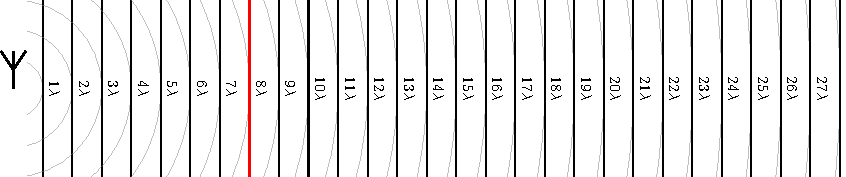
\includegraphics{../pictures/plana_0.pdf}
    \caption*{Fonte: Autor.}
    \label{fig:plana_0}
\end{figure}


Tomando agora um par de antenas separadas por uma distância fixa $d$, torna-se viável fazer a análise trigonométrica entre as antenas e a frente de onda que chega, onde essa distância $d$ será a hipotenusa do triângulo.
A \autoref{fig:AoA} apresenta a disposição das antenas em quatro casos de chegada de sinal \ac{RF}.
Para realizar a análise, é necessário conhecer uma segunda dimensão do triângulo retângulo envolvido, esta é obtida analisando a defasagem entre o sinal das antenas, conforme apresentado na \autoref{eq:defasagem}.


\begin{equation} \label{eq:defasagem} % Relação trigonometrica de defasagem e angulo do sinal
    d \cdot \cos\left(\pm\beta\right) = \lambda \cdot \frac{\Delta\Phi}{2 \pi}
\end{equation}


É importante ressaltar que um sistemas com um único par de antenas não é capaz de determinar completamente o \ac{AoA}, já que o valor calculado de $\beta$ é igual para casos simétricos, a relação é apresentada nas Figuras \ref{fig:AoA:1} e \ref{fig:AoA:2}.
Existem ainda dois casos notáveis, onde o sinal chega alinhado com o par de antenas ou perpendicular a elas, apresentados respectivamente nas Figuras \ref{fig:AoA:3} e \ref{fig:AoA:4}.

\begin{figure}
    \caption{\ac{AoA} ($\Theta$) com par de antenas em diversas direções equivalentes, sistema com ângulo $\alpha=\SI{20}{\degree}$.}
    \label{fig:AoA}

    \hfill
    \begin{subfigure}[b]{0.45\textwidth}
        \centering
        \caption{$\Theta=\SI{60}{\degree}$, $\beta=\SI{40}{\degree}$}
        % \resizebox{!}{0.7\textheight}{%
\begin{circuitikz}[american, voltage shift=0.5, line width=0.5, every node/.style={font = {\footnotesize\bfseries}}]

    \def\wavelength{3.5}
    \pgfmathsetmacro\d{0.5*\wavelength}

    \def\antennaAngle{20}
    \pgfmathsetmacro\signalAngle{\antennaAngle+40}

    \def\closeRange{9}
    \def\farRange{\closeRange+13}

	\def\NAntennas{3}
	\pgfmathsetmacro\AngleAntennas{360/\NAntennas}
	\def\ShiftAngleAntennas{-90}

	\pgfmathsetmacro\RhoAntennas{\d/(2*sin(180/\NAntennas))}

    \def\centerarc(#1)(#2:#3:#4)% Syntax: [draw options] (center) (initial angle:final angle:radius)
    { ($(#1)+({#4*cos(#2)},{#4*sin(#2)})$) arc (#2:#3:#4) }

    \def\coordref[#1](#2){%

        \coordinate(sysref) at (#2);

        \draw[#1, -latex] (sysref) ++(-0.4,-0.3) -- ++(0.9,0) node[midway, below]{$x$};
        \draw[#1, -latex] (sysref) ++(-0.3,-0.4) -- ++(0,0.9) node[midway, left]{$y$};
        \draw[#1, -latex] \centerarc(sysref)(-90:180:0.25);
        \draw[#1] (sysref) node{$+$}
    }

    \coordinate (bottomleft) at (-3.5,-1);
    \coordinate (topright) at (3.5,5);


    % \draw[Red,dashed] (bottomleft) rectangle (topright);
    \clip (bottomleft) rectangle (topright);

    \coordinate (O) at (0,0);
    \coordinate (sourceAntenna) at (\signalAngle:\closeRange*\wavelength);
    % \draw [help lines, dashed] (bottomleft) grid (topright); % desenha grid
    % \draw [red] (O) node[draw,cross out] {}; % marca pont(0,0)

    % Circulo de antenas
	% \draw[densely dotted, opacity=0.25] (O) ++(90:\RhoAntennas) circle (\RhoAntennas);

    % Linhas do sinal de fundo
    \foreach \x [evaluate={\y=int((\x+\closeRange));\z=int((\x+\closeRange));}] in {-3,...,3} {
        \draw [black!75, very thin]
        (sourceAntenna) ++ (\signalAngle:-\z*\wavelength)
            % node[anchor=west, font = {\footnotesize\bfseries}]{$\y\lambda$}
        ($(sourceAntenna) + (\signalAngle:-\z*\wavelength) + ({10*cos(\signalAngle+90)},{10*sin(\signalAngle+90)})$)
            --
        ($(sourceAntenna) + (\signalAngle:-\z*\wavelength) - ({10*cos(\signalAngle+90)},{10*sin(\signalAngle+90)})$)
        % \draw [gray, thin] (sourceAntenna) circle (\z)
        ;
    }

    % Antenas
    \draw[thick, cmyk_R] (O) node[dinantenna] (A00) {} ;
    % \draw[thick, cmyk_G, opacity=0.75] (O) ++(60:\d) node[dinantenna] (A0d) {} node [below] {$A_{k+2}$};
    \draw[thick, cmyk_B] (O) ++(\antennaAngle:\d) node[dinantenna] (Ad0) {} ;

    \draw[very thin, Black!50, -latex] % Desenha eixo X
        (-3,0) -- (3,0) node[below left] {$x$}
    ;

    % Ângulo alpha entre antenas
    \draw[thin, cmyk_M]
        \centerarc(O)(0:\antennaAngle:0.3)
        node [above, inner sep=3pt] {$\alpha$}
    ;


    % Desenha senoide de fundo
    \draw[Goldenrod, domain=-8:8, samples=100]
        (A00) ++(\signalAngle+90:0.5*\wavelength) coordinate(signalAux)
        plot[shift={(signalAux)}, rotate=\signalAngle]({\x},{cos(\x * pi * 2 / \wavelength r)})
    ;

    % Direção do sinal
    \draw[very thick, dashed, -latex, Goldenrod]
        % (A00) ++(1.5*\d,0) ++ (\signalAngle:-0.5*\d) -- coordinate(angleArrow) ++(\signalAngle:\d)
        (A00) ++(-2,0) ++ (\signalAngle:-0.25*\d) -- coordinate(angleArrow) ++ (\signalAngle:0.5*\d) --++(\signalAngle:0.25*\d)
    ;
    % Angulo Theta do sinal
    \draw[thin]
        (angleArrow) ++ (0.4, 0) node [below,inner sep=2pt] {$\Theta$}
        \centerarc(angleArrow)(0:\signalAngle:0.4)
    ;

    % Triangulo retângulo + quadradinho
    \draw[Black]

        (A00) --++($({\signalAngle-90}:{\d*sin(\signalAngle-\antennaAngle)})$) coordinate (pontoTriangulo) -- (Ad0) -- (A00)

        (pontoTriangulo)
          ++(\signalAngle:0.125)
        --++(\signalAngle+90:0.125)
        --++(\signalAngle+180:0.125)
    ;

    % Arco do angulo beta
    \draw[thin]
        (Ad0) ++ (180+\antennaAngle:0.4) node[above, inner sep=3pt] {$\beta$}
        \centerarc(Ad0)(180+\antennaAngle:180+\signalAngle:0.4)
    ;

    % Distânci d entre antenas
    \draw[latex-latex]
        ($(A00)+(0,1)$) -- ($(Ad0)+(0,1)$) node [midway, fill=white, circle, inner sep=1pt] {$d$}
    ;

    \newcommand\CircleRadius{3cm}
    %   \draw (0,0) circle (\CircleRadius);
    % special method of noting the position of a point
    \coordinate (P) at (50:\CircleRadius);

\end{circuitikz}
% }


        % 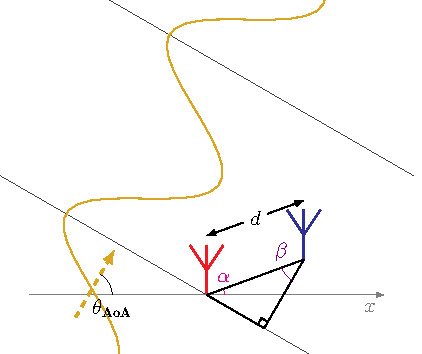
\includegraphics{../pictures/AoA_1.pdf}
        \label{fig:AoA:1}
    \end{subfigure}
    \hfill
    \begin{subfigure}[b]{0.45\textwidth}
        \centering
        \caption{$\Theta=\SI{-20}{\degree}$, $\beta=\SI{40}{\degree}$}
        % \resizebox{!}{0.7\textheight}{%
\begin{circuitikz}[american, voltage shift=0.5, line width=0.5, every node/.style={font = {\footnotesize\bfseries}}]

    \def\wavelength{3.5}
    \pgfmathsetmacro\d{0.5*\wavelength}

    \def\antennaAngle{20}
    \pgfmathsetmacro\signalAngle{\antennaAngle-40}

    \def\closeRange{9}
    \def\farRange{\closeRange+13}

	\def\NAntennas{3}
	\pgfmathsetmacro\AngleAntennas{360/\NAntennas}
	\def\ShiftAngleAntennas{-90}

	\pgfmathsetmacro\RhoAntennas{\d/(2*sin(180/\NAntennas))}

    \def\centerarc(#1)(#2:#3:#4)% Syntax: [draw options] (center) (initial angle:final angle:radius)
    { ($(#1)+({#4*cos(#2)},{#4*sin(#2)})$) arc (#2:#3:#4) }

    \def\coordref[#1](#2){%

        \coordinate(sysref) at (#2);

        \draw[#1, -latex] (sysref) ++(-0.4,-0.3) -- ++(0.9,0) node[midway, below]{$x$};
        \draw[#1, -latex] (sysref) ++(-0.3,-0.4) -- ++(0,0.9) node[midway, left]{$y$};
        \draw[#1, -latex] \centerarc(sysref)(-90:180:0.25);
        \draw[#1] (sysref) node{$+$}
    }

    \coordinate (bottomleft) at (-3.5,-1);
    \coordinate (topright) at (3.5,5);


    % \draw[Red,dashed] (bottomleft) rectangle (topright);
    \clip (bottomleft) rectangle (topright);

    \coordinate (O) at (0,0);
    \coordinate (sourceAntenna) at (\signalAngle:\closeRange*\wavelength);
    % \draw [help lines, dashed] (bottomleft) grid (topright); % desenha grid
    % \draw [red] (O) node[draw,cross out] {}; % marca pont(0,0)

    % Circulo de antenas
	% \draw[densely dotted, opacity=0.25] (O) ++(90:\RhoAntennas) circle (\RhoAntennas);

    % Linhas do sinal de fundo
    \foreach \x [evaluate={\y=int((\x+\closeRange));\z=int((\x+\closeRange));}] in {-3,...,3} {
        \draw [black!75, very thin]
        (sourceAntenna) ++ (\signalAngle:-\z*\wavelength)
            % node[anchor=west, font = {\footnotesize\bfseries}]{$\y\lambda$}
        ($(sourceAntenna) + (\signalAngle:-\z*\wavelength) + ({10*cos(\signalAngle+90)},{10*sin(\signalAngle+90)})$)
            --
        ($(sourceAntenna) + (\signalAngle:-\z*\wavelength) - ({10*cos(\signalAngle+90)},{10*sin(\signalAngle+90)})$)
        % \draw [gray, thin] (sourceAntenna) circle (\z)
        ;
    }

    % Antenas
    \draw[thick, cmyk_R] (O) node[dinantenna] (A00) {} ;
    % \draw[thick, cmyk_G, opacity=0.75] (O) ++(60:\d) node[dinantenna] (A0d) {} node [below] {$A_{k+2}$};
    \draw[thick, cmyk_B] (O) ++(\antennaAngle:\d) node[dinantenna] (Ad0) {} ;

    \draw[very thin, Black!50, -latex] % Desenha eixo X
        (-3,0) -- (3,0) node[below left] {$x$}
    ;

    % Ângulo alpha entre antenas
    \draw[thin, cmyk_M]
		(0.3,0) node [below, inner sep=3pt] {$\alpha$}
		\centerarc(O)(0:\antennaAngle:0.3)
    ;


    % Desenha senoide de fundo
    \draw[Goldenrod, domain=-8:8, samples=100]
        (A00) ++(\signalAngle+90:0.8*\wavelength) coordinate(signalAux)
        plot[shift={(signalAux)}, rotate=\signalAngle]({\x},{cos(\x * pi * 2 / \wavelength r)})
    ;

    % Direção do sinal
    \draw[very thick, dashed, -latex, Goldenrod]
		% (A00) ++(1.5*\d,0) ++ (\signalAngle:-0.25*\d) -- coordinate(angleArrow) ++(\signalAngle:0.85*\d)
        (A00) ++(-2,0) ++ (\signalAngle:-0.25*\d) -- coordinate(angleArrow) ++ (\signalAngle:0.5*\d) --++(\signalAngle:0.25*\d)
    ;
    % Angulo Theta do sinal
    \draw[thin]
        (angleArrow) ++ (0.4, 0) node [above,inner sep=2pt] {$\Theta$}
        \centerarc(angleArrow)(0:\signalAngle:0.4)
    ;

    % Triangulo retângulo + quadradinho
    \draw[Black]

        (A00) --++($({\signalAngle-90}:{\d*sin(\signalAngle-\antennaAngle)})$) coordinate (pontoTriangulo) -- (Ad0) -- (A00)

        (pontoTriangulo)
          ++(\signalAngle:0.125)
        --++(\signalAngle-90:0.125)
        --++(\signalAngle+180:0.125)
    ;

    % Arco do angulo beta
    \draw[thin]
        \centerarc(Ad0)(180+\antennaAngle:180+\signalAngle:0.4)
		(Ad0) ++ (180+\antennaAngle:0.4) node[below, inner sep=3pt] {$\beta$}
    ;

    % Distânci d entre antenas
    \draw[latex-latex]
        ($(A00)+(0,1)$) -- ($(Ad0)+(0,1)$) node [midway, fill=white, circle, inner sep=1pt] {$d$}
    ;

    \newcommand\CircleRadius{3cm}
    %   \draw (0,0) circle (\CircleRadius);
    % special method of noting the position of a point
    \coordinate (P) at (50:\CircleRadius);

\end{circuitikz}
% }


        % 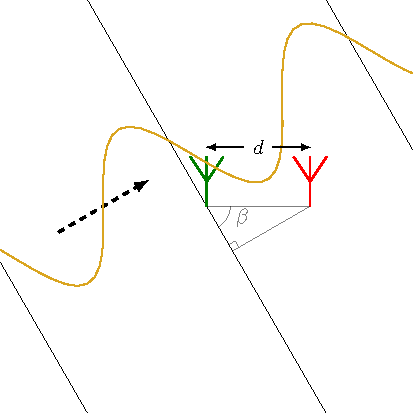
\includegraphics{../pictures/AoA_2.pdf}
        \label{fig:AoA:2}
    \end{subfigure}
    \hfill

    \vspace{\floatsep}

    \hfill
    \begin{subfigure}[b]{0.45\textwidth}
        \centering
        \caption{$\Theta=\SI{110}{\degree}$, $\beta=\SI{90}{\degree}$}
        % \resizebox{!}{0.7\textheight}{%
\begin{circuitikz}[american, voltage shift=0.5, line width=0.5, every node/.style={font = {\footnotesize\bfseries}}]

    \def\wavelength{3.5}
    \pgfmathsetmacro\d{0.5*\wavelength}

    \def\antennaAngle{20}
    \pgfmathsetmacro\signalAngle{\antennaAngle+90}

    \def\closeRange{9}
    \def\farRange{\closeRange+13}

	\def\NAntennas{3}
	\pgfmathsetmacro\AngleAntennas{360/\NAntennas}
	\def\ShiftAngleAntennas{-90}

	\pgfmathsetmacro\RhoAntennas{\d/(2*sin(180/\NAntennas))}

    \def\centerarc(#1)(#2:#3:#4)% Syntax: [draw options] (center) (initial angle:final angle:radius)
    { ($(#1)+({#4*cos(#2)},{#4*sin(#2)})$) arc (#2:#3:#4) }

    \def\coordref[#1](#2){%

        \coordinate(sysref) at (#2);

        \draw[#1, -latex] (sysref) ++(-0.4,-0.3) -- ++(0.9,0) node[midway, below]{$x$};
        \draw[#1, -latex] (sysref) ++(-0.3,-0.4) -- ++(0,0.9) node[midway, left]{$y$};
        \draw[#1, -latex] \centerarc(sysref)(-90:180:0.25);
        \draw[#1] (sysref) node{$+$}
    }

    \coordinate (bottomleft) at (-3.5,-1);
    \coordinate (topright) at (3.5,5);


    % \draw[Red,dashed] (bottomleft) rectangle (topright);
    \clip (bottomleft) rectangle (topright);

    \coordinate (O) at (0,0);
    \coordinate (sourceAntenna) at (\signalAngle:\closeRange*\wavelength);
    % \draw [help lines, dashed] (bottomleft) grid (topright); % desenha grid
    % \draw [red] (O) node[draw,cross out] {}; % marca pont(0,0)

    % Circulo de antenas
	% \draw[densely dotted, opacity=0.25] (O) ++(90:\RhoAntennas) circle (\RhoAntennas);

    % Linhas do sinal de fundo
    \foreach \x [evaluate={\y=int((\x+\closeRange));\z=int((\x+\closeRange));}] in {-3,...,3} {
        \draw [black!75, very thin]
        (sourceAntenna) ++ (\signalAngle:-\z*\wavelength)
            % node[anchor=west, font = {\footnotesize\bfseries}]{$\y\lambda$}
        ($(sourceAntenna) + (\signalAngle:-\z*\wavelength) + ({10*cos(\signalAngle+90)},{10*sin(\signalAngle+90)})$)
            --
        ($(sourceAntenna) + (\signalAngle:-\z*\wavelength) - ({10*cos(\signalAngle+90)},{10*sin(\signalAngle+90)})$)
        % \draw [gray, thin] (sourceAntenna) circle (\z)
        ;
    }

    % Antenas
    \draw[thick, cmyk_R] (O) node[dinantenna] (A00) {} ;
    % \draw[thick, cmyk_G, opacity=0.75] (O) ++(60:\d) node[dinantenna] (A0d) {} node [below] {$A_{k+2}$};
    \draw[thick, cmyk_B] (O) ++(\antennaAngle:\d) node[dinantenna] (Ad0) {} ;

    \draw[very thin, Black!50, -latex] % Desenha eixo X
        (-3,0) -- (3,0) node[below left] {$x$}
    ;

    % Ângulo alpha entre antenas
    \draw[thin, cmyk_M]
		(0.3,0) node [below, inner sep=3pt] {$\alpha$}
		\centerarc(O)(0:\antennaAngle:0.3)
    ;


    % Desenha senoide de fundo
    \draw[Goldenrod, domain=-8:8, samples=100]
        (A00) ++(\signalAngle+90:0.25*\d) coordinate(signalAux)
        plot[shift={(signalAux)}, rotate=\signalAngle]({\x},{cos(\x * pi * 2 / \wavelength r)})
    ;

    % Direção do sinal
    \draw[very thick, dashed, -latex, Goldenrod]
		% (A00) ++(1.5*\d,0) ++ (\signalAngle:-0.25*\d) -- coordinate(angleArrow) ++(\signalAngle:0.85*\d)
        (A00) ++(-2,0) ++ (\signalAngle:-0.25*\d) -- coordinate(angleArrow) ++ (\signalAngle:0.5*\d) --++(\signalAngle:0.25*\d)
    ;
    % Angulo Theta do sinal
    \draw[thin]
        (angleArrow) ++ (0.4, 0) node [below,inner sep=2pt] {$\Theta$}
        \centerarc(angleArrow)(0:\signalAngle:0.4)
    ;

    % % Triangulo retângulo + quadradinho
    % \draw[Black]

    %     % (A00) --++($({\signalAngle-90}:{\d*sin(\signalAngle-\antennaAngle)})$) coordinate (pontoTriangulo) --
	% 	% (Ad0) -- (A00)

    %     % (pontoTriangulo)
    %     %   ++(\signalAngle:0.125)
    %     % --++(\signalAngle+90:0.125)
    %     % --++(\signalAngle+180:0.125)
    % ;

    % % Arco do angulo beta
    % \draw[thin]
    %     \centerarc(Ad0)(180+\antennaAngle:180+\signalAngle:0.4) node[below, inner sep=3pt] {$\beta$}
    % ;

    % Distânci d entre antenas
    \draw[latex-latex]
        ($(A00)+(0,1)$) -- ($(Ad0)+(0,1)$) node [midway, fill=white, circle, inner sep=1pt] {$d$}
    ;

    \newcommand\CircleRadius{3cm}
    %   \draw (0,0) circle (\CircleRadius);
    % special method of noting the position of a point
    \coordinate (P) at (50:\CircleRadius);

\end{circuitikz}
% }


        % 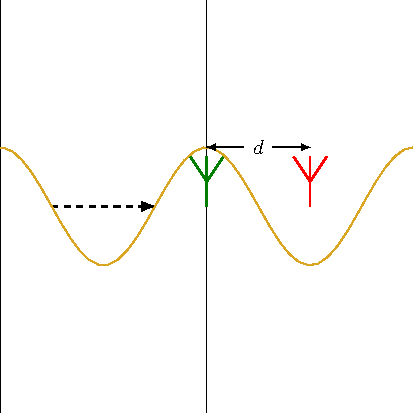
\includegraphics{../pictures/AoA_3.pdf}
        \label{fig:AoA:3}
    \end{subfigure}
    \hfill
    \begin{subfigure}[b]{0.45\textwidth}
        \centering
        \caption{$\Theta=\SI{20}{\degree}$, $\beta=\SI{0}{\degree}$}
        % \resizebox{!}{0.7\textheight}{%
\begin{circuitikz}[american, voltage shift=0.5, line width=0.5, every node/.style={font = {\footnotesize\bfseries}}]

    \def\wavelength{3.5}
    \pgfmathsetmacro\d{0.5*\wavelength}

    \def\antennaAngle{20}
    \def\signalAngle{\antennaAngle}

    \def\closeRange{9}
    \def\farRange{\closeRange+13}

	\def\NAntennas{3}
	\pgfmathsetmacro\AngleAntennas{360/\NAntennas}
	\def\ShiftAngleAntennas{-90}

	\pgfmathsetmacro\RhoAntennas{\d/(2*sin(180/\NAntennas))}

    \def\centerarc(#1)(#2:#3:#4)% Syntax: [draw options] (center) (initial angle:final angle:radius)
    { ($(#1)+({#4*cos(#2)},{#4*sin(#2)})$) arc (#2:#3:#4) }

    \def\coordref[#1](#2){%

        \coordinate(sysref) at (#2);

        \draw[#1, -latex] (sysref) ++(-0.4,-0.3) -- ++(0.9,0) node[midway, below]{$x$};
        \draw[#1, -latex] (sysref) ++(-0.3,-0.4) -- ++(0,0.9) node[midway, left]{$y$};
        \draw[#1, -latex] \centerarc(sysref)(-90:180:0.25);
        \draw[#1] (sysref) node{$+$}
    }

    \coordinate (bottomleft) at (-3.5,-1);
    \coordinate (topright) at (3.5,5);


    % \draw[Red,dashed] (bottomleft) rectangle (topright);
    \clip (bottomleft) rectangle (topright);

    \coordinate (O) at (0,0);
    \coordinate (sourceAntenna) at (\signalAngle:\closeRange*\wavelength);
    % \draw [help lines, dashed] (bottomleft) grid (topright); % desenha grid
    % \draw [red] (O) node[draw,cross out] {}; % marca pont(0,0)

    % Circulo de antenas
	% \draw[densely dotted, opacity=0.25] (O) ++(90:\RhoAntennas) circle (\RhoAntennas);

    % Linhas do sinal de fundo
    \foreach \x [evaluate={\y=int((\x+\closeRange));\z=int((\x+\closeRange));}] in {-3,...,3} {
        \draw [black!75, very thin]
        (sourceAntenna) ++ (\signalAngle:-\z*\wavelength)
            % node[anchor=west, font = {\footnotesize\bfseries}]{$\y\lambda$}
        ($(sourceAntenna) + (\signalAngle:-\z*\wavelength) + ({10*cos(\signalAngle+90)},{10*sin(\signalAngle+90)})$)
            --
        ($(sourceAntenna) + (\signalAngle:-\z*\wavelength) - ({10*cos(\signalAngle+90)},{10*sin(\signalAngle+90)})$)
        % \draw [gray, thin] (sourceAntenna) circle (\z)
        ;
    }

    % Antenas
    \draw[thick, cmyk_R] (O) node[dinantenna] (A00) {} ;
    % \draw[thick, cmyk_G, opacity=0.75] (O) ++(60:\d) node[dinantenna] (A0d) {} node [below] {$A_{k+2}$};
    \draw[thick, cmyk_B] (O) ++(\antennaAngle:\d) node[dinantenna] (Ad0) {} ;

    \draw[very thin, Black!50, -latex] % Desenha eixo X
        (-3,0) -- (3,0) node[below left] {$x$}
    ;

    % Ângulo alpha entre antenas
    \draw[thin, cmyk_M]
		(0.3,0) node [below, inner sep=3pt] {$\alpha$}
		\centerarc(O)(0:\antennaAngle:0.3)
    ;


    % Desenha senoide de fundo
    \draw[Goldenrod, domain=-8:8, samples=100]
        (A00) ++(\signalAngle+90:0.75*\wavelength) coordinate(signalAux)
        plot[shift={(signalAux)}, rotate=\signalAngle]({\x},{cos(\x * pi * 2 / \wavelength r)})
    ;

    % Direção do sinal
    \draw[very thick, dashed, -latex, Goldenrod]
        % (A00) ++(1.5*\d,0) ++ (\signalAngle:-0.25*\d) -- coordinate(angleArrow) ++(\signalAngle:0.85*\d)
        (A00) ++(-2,0) ++ (\signalAngle:-0.25*\d) -- coordinate(angleArrow) ++ (\signalAngle:0.5*\d) --++(\signalAngle:0.25*\d)
    ;
    % Angulo Theta do sinal
    \draw[thin]
        (angleArrow) ++ (0.4, 0) node [below,inner sep=2pt] {$\theta_\text{\ac{AoA}}$}
        \centerarc(angleArrow)(0:\signalAngle:0.4)
    ;

    % Triangulo retângulo + quadradinho
    \draw[Black]

    %     % (A00) --++($({\signalAngle-90}:{\d*sin(\signalAngle-\antennaAngle)})$) coordinate (pontoTriangulo) --
		(Ad0) -- (A00)

    %     % (pontoTriangulo)
    %     %   ++(\signalAngle:0.125)
    %     % --++(\signalAngle+90:0.125)
    %     % --++(\signalAngle+180:0.125)
    ;

    % % Arco do angulo beta
    % \draw[thin]
    %     \centerarc(Ad0)(180+\antennaAngle:180+\signalAngle:0.4) node[below, inner sep=3pt] {$\beta$}
    % ;

    % Distânci d entre antenas
    \draw[latex-latex]
        ($(A00)+(0,1)$) -- ($(Ad0)+(0,1)$) node [midway, fill=white, circle, inner sep=1pt] {$d$}
    ;

    \newcommand\CircleRadius{3cm}
    %   \draw (0,0) circle (\CircleRadius);
    % special method of noting the position of a point
    \coordinate (P) at (50:\CircleRadius);

\end{circuitikz}
% }


        % 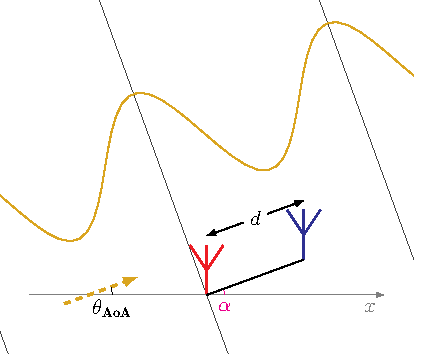
\includegraphics{../pictures/AoA_4.pdf}
        \label{fig:AoA:4}
    \end{subfigure}
    \hfill

    \caption*{Fonte: Autor.}
\end{figure}

A escolha da distância $d$ entre as antenas deve ser feita de forma a otimizar a resolução da medida de defasagem, com a maior distância possível. Porém é necessário evitar ambiguidades na análise, como o sinal é periódico, o valor se repetirá a cada $\lambda$, e terá valores simétricos quando $d > \sfrac{\lambda}{2}$, ilustrado na \autoref{fig:AoA_d:fail}.
Adota-se então $d=\sfrac{\lambda}{2}$, conforme apresentado na \autoref{fig:AoA_d:ok} \cite{bensky2016wireless, horst2021localization}.

\begin{figure}
    \caption{Diferentes valores para $d$.}
    \label{fig:AoA_d}

    \hfill
    \begin{subfigure}[b]{0.45\textwidth}
        \centering
        \caption{$d > \sfrac{\lambda}{2}$}
        %     % \resizebox{!}{0.7\textheight}{%
    \begin{circuitikz}[american, voltage shift=0.5, line width=0.5,every node/.style={font = {\footnotesize\bfseries}}]

        \def\wavelength{4}
        \def\d{0.5*\wavelength}


        \def\antennaAngle{120}
        \def\closeRange{9}
        \def\farRange{\closeRange+13}

        \def\centerarc[#1](#2)(#3:#4:#5)% Syntax: [draw options] (center) (initial angle:final angle:radius)
        { \draw[#1] ($(#2)+({#5*cos(#3)},{#5*sin(#3)})$) arc (#3:#4:#5) node[midway,anchor=west] {$\beta$}; }


        \coordinate (O) at (0,0);
        \coordinate (antenna) at (\antennaAngle:\closeRange*\wavelength);
        % \draw [help lines, dashed] (-3,-3) grid (3,3); % desenha grid
        % \draw [red] (O) node[draw,cross out] {}; % marca pont(0,0)

        % \draw (-6.8,-4) rectangle (6.8,4);
        \clip (-1,-1.1) rectangle (5,1.1);


        \draw[thick]
            (0,0)  node[cmyk_B, dinantenna] (A00) {}
            % (0,\d) node[Blue,  dinantenna] (A0d) {}
            (1.2*\d,0) node[cmyk_R,   dinantenna] (Ad0) {}
            (0.8*\d,0) node[cmyk_R,   dinantenna, opacity=0.2] (Ad0_phantom) {}
        ;

        % \draw[Goldenrod, domain=-3:3, samples=100] plot[shift={(-1,-1)}, rotate=30]({\x},{sin(\x * pi * 2 / \wavelength r)});
        \draw[Goldenrod, domain=-3:6, samples=50]
            plot ({\x},{cos(\x * pi * 2 / \wavelength r)})
        ;

        \draw[Black, dashed, domain=-3:6, samples=2]
            plot[Black, thin, dashed, samples=2] (\x,0)
        ;

        \draw [densely dotted, cmyk_R]
            (Ad0_phantom) --
            ++(0,{cos(1.2*\d * pi * 2 / \wavelength r)}) --
            ++({0.4*\d},0) --
            (Ad0)
        ;

    \end{circuitikz}
  % }
        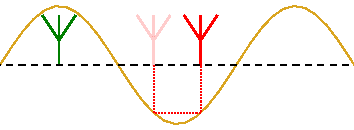
\includegraphics{../pictures/AoA_0_fail.pdf}
        \label{fig:AoA_d:fail}
    \end{subfigure}
    \hfill
    \begin{subfigure}[b]{0.45\textwidth}
        \centering
        \caption{$d = \sfrac{\lambda}{2}$}
        %     % \resizebox{!}{0.7\textheight}{%
    \begin{circuitikz}[american, voltage shift=0.5, line width=0.5,every node/.style={font = {\footnotesize\bfseries}}]

        \def\wavelength{4}
        \def\d{0.5*\wavelength}


        \def\antennaAngle{120}
        \def\closeRange{9}
        \def\farRange{\closeRange+13}

        \def\centerarc[#1](#2)(#3:#4:#5)% Syntax: [draw options] (center) (initial angle:final angle:radius)
        { \draw[#1] ($(#2)+({#5*cos(#3)},{#5*sin(#3)})$) arc (#3:#4:#5) node[midway,anchor=west] {$\beta$}; }


        \coordinate (O) at (0,0);
        \coordinate (antenna) at (\antennaAngle:\closeRange*\wavelength);
        % \draw [help lines, dashed] (-3,-3) grid (3,3); % desenha grid
        % \draw [red] (O) node[draw,cross out] {}; % marca pont(0,0) 
        
        % \draw (5,1.25) rectangle (-1,-1.1);
        \clip (5,1.25) rectangle (-1,-1.1);

        
        % \draw[Goldenrod, domain=-3:3, samples=100] plot[shift={(-1,-1)}, rotate=30]({\x},{sin(\x * pi * 2 / \wavelength r)});
        \draw[Goldenrod, domain=-3:6, samples=50] 
            plot ({\x},{cos(\x * pi * 2 / \wavelength r)})
        ;
        
        \draw[Black, dashed, domain=-3:6, samples=2] 
            plot[Black, thin, dashed, samples=2] (\x,0)
        ;
        
        
        % \pause
        \draw[thick]
            (0,0)  node[Green, dinantenna] (A00) {}
            % (0,\d) node[Blue,  dinantenna] (A0d) {}
            % (\d,0) node[Red,   dinantenna] (Ad0) {}
        ;
        
        % \pause
        \draw[thick]
            % (0,0)  node[Green, dinantenna] (A00) {}
            % (0,\d) node[Blue,  dinantenna] (A0d) {}
            (\d,0) node[Red,   dinantenna] (Ad0) {}
        ;

        \draw[latex-latex]
            ($(A00)+(0,1.1)$) -- ++(\wavelength,0) node [midway, fill=white] {$\lambda$}
        ;
    % \visible<7->{
        \draw[latex-latex]
            ($(A00)+(0,-0.1)$) -- ++(0.5*\wavelength,0) node [midway, fill=white, fill opacity=0.75, anchor=north] {$d = \sfrac{\lambda}{2}$}
        ;
    % }
            
    \end{circuitikz}
  % }
        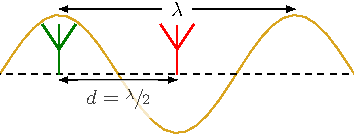
\includegraphics{../pictures/AoA_0.pdf}
        \label{fig:AoA_d:ok}
    \end{subfigure}
    \hfill

    \caption*{Fonte: Autor.}
\end{figure}


















\begin{figure}[H]
    \centering
    % \resizebox{!}{0.7\textheight}{%
\begin{circuitikz}[american, voltage shift=0.5, line width=0.5,every node/.style={font = {\footnotesize\bfseries}}]

    \def\wavelength{8}
    \pgfmathsetmacro\d{0.5*\wavelength}

    \def\signalAngle{75}
    \def\antennaAngle{120}

    \def\closeRange{9}
    \def\farRange{\closeRange+13}

	\def\NAntennas{3}
	\pgfmathsetmacro\AngleAntennas{360/\NAntennas}
	\def\ShiftAngleAntennas{-90}

	\pgfmathsetmacro\RhoAntennas{\d/(2*sin(180/\NAntennas))}

    \def\centerarc(#1)(#2:#3:#4)% Syntax: [draw options] (center) (initial angle:final angle:radius)
    { ($(#1)+({#4*cos(#2)},{#4*sin(#2)})$) arc (#2:#3:#4) }

    \def\coordref[#1](#2){%

        \coordinate(sysref) at (#2);

        \draw[#1, -latex] (sysref) ++(-0.4,-0.3) -- ++(0.9,0) node[midway, below]{$x$};
        \draw[#1, -latex] (sysref) ++(-0.3,-0.4) -- ++(0,0.9) node[midway, left]{$y$};
        \draw[#1, -latex] \centerarc(sysref)(-90:180:0.25);
        \draw[#1] (sysref) node{$+$}
    }

    \coordinate (bottomleft) at (-6,-3);
    \coordinate (topright) at (6,3);


    % \draw[Red,dashed] (bottomleft) rectangle (topright);
    \clip (bottomleft) rectangle (topright);

    \coordinate (O) at (0,0);
    \coordinate (sourceAntenna) at (\signalAngle:\closeRange*\wavelength);
    % \draw [help lines, dashed] (bottomleft) grid (topright); % desenha grid
    % \draw [red] (O) node[draw,cross out] {}; % marca pont(0,0)

	\draw[densely dotted] (O) circle (\RhoAntennas);

    \draw[thick, cmyk_G] (O) ++(1*\AngleAntennas+\ShiftAngleAntennas:\RhoAntennas) node[dinantenna] (A1) {} node [above right] {$A_{k+2}$};
    \draw[thick, cmyk_B] (O) ++(2*\AngleAntennas+\ShiftAngleAntennas:\RhoAntennas) node[dinantenna] (A2) {} node [above left] {$A_{k}$};
    \draw[thick, cmyk_R] (O) ++(3*\AngleAntennas+\ShiftAngleAntennas:\RhoAntennas) node[dinantenna] (A3) {} node [below] {$A_{k+1}$};

	\coordinate (A1_2) at ($(A1)!0.5!(A2)$);

	\draw[Black!25, dotted]
		(A1) --
		(A3) --
		(A2)
	;

	\draw[Black!50, densely dotted]
		(O) --
		(A2) --
		(A1_2)
	;

	\draw
		(A1) --
		(O) --
		(A1_2) --
		(A1)
	;

	\draw
         (A1_2)
           ++(0:0.125)
         --++(-90:0.125)
         --++(+180:0.125)
	;

	\node at (O) {\tiny\textbullet};

	\draw
		(O) ++(90:0.3) node[above right, inner sep=1.5pt] {$\textstyle \frac{\pi}{N_\text{ant}}$}
		\centerarc(O)(1*\AngleAntennas+\ShiftAngleAntennas:90:0.3)
	;


    % Distânci d entre antenas
    \draw[latex-latex]
        ($(A1)+(0,1)$) -- ($(A2)+(0,1)$) node [midway, fill=white, circle, inner sep=1pt] {$d$}
    ;

    \draw[decorate, decoration={brace, amplitude=5pt}, thin]
    ($(A1)+({1*\AngleAntennas+\ShiftAngleAntennas-90}:0.1)$)
    -- coordinate (brace)
    ($(O)+({1*\AngleAntennas+\ShiftAngleAntennas-90}:0.1)$)
    ;

    \draw (brace) ++({1*\AngleAntennas+\ShiftAngleAntennas-90}:5pt)
        node[anchor=north west, circle, fill=white, inner sep=1pt] {$\rho$}
    ;

	\draw[decorate, decoration={brace, amplitude=5pt}, thin]
    ($(A1_2)+({90}:0.1)$)
    -- coordinate (brace)
    ($(A1)+({90}:0.1)$)
    ;

    \draw (brace) ++({90}:5pt)
        node[anchor=south, circle, inner sep=1pt] {$\sfrac{d}{2}$}
    ;

    \coordref[Black!25](3.5,0);

\end{circuitikz}
% }


    \caption{Agora sim 0}
\end{figure}

\begin{figure}[H]
    \centering
    % \resizebox{!}{0.7\textheight}{%
\begin{circuitikz}[american, voltage shift=0.5, line width=0.5,every node/.style={font = {\footnotesize\bfseries}}]

    \def\wavelength{5}
    \pgfmathsetmacro\d{0.5*\wavelength}

    \def\signalAngle{75}
    \def\antennaAngle{120}

    \def\closeRange{9}
    \def\farRange{\closeRange+13}

	\def\NAntennas{3}
	\pgfmathsetmacro\AngleAntennas{360/\NAntennas}
	\def\ShiftAngleAntennas{-90}

	\pgfmathsetmacro\RhoAntennas{\d/(2*sin(180/\NAntennas))}

    % \def\centerarc[#1](#2)(#3:#4:#5)% Syntax: [draw options] (center) (initial angle:final angle:radius)
    % { \draw[#1] ($(#2)+({#5*cos(#3)},{#5*sin(#3)})$) arc (#3:#4:#5) node[midway,anchor=east] {$\beta$}; }
    \def\centerarc(#1)(#2:#3:#4)% Syntax: [draw options] (center) (initial angle:final angle:radius)
    { ($(#1)+({#4*cos(#2)},{#4*sin(#2)})$) arc (#2:#3:#4) }

    \def\coordref[#1](#2){%

        \coordinate(sysref) at (#2);

        \draw[#1, -latex] (sysref) ++(-0.4,-0.3) -- ++(0.9,0) node[midway, below]{$x$};
        \draw[#1, -latex] (sysref) ++(-0.3,-0.4) -- ++(0,0.9) node[midway, left]{$y$};
        \draw[#1, -latex] \centerarc(sysref)(-90:180:0.25);
        \draw[#1] (sysref) node{$+$}
    }

    \coordinate (bottomleft) at (-6,-0.5);
    \coordinate (topright) at (6,6.5);


    % \draw[Red,dashed] (bottomleft) rectangle (topright);
    \clip (bottomleft) rectangle (topright);

    \coordinate (O) at (0,0);
    \coordinate (sourceAntenna) at (\signalAngle:\closeRange*\wavelength);
    % \draw [help lines, dashed] (bottomleft) grid (topright); % desenha grid
    % \draw [red] (O) node[draw,cross out] {}; % marca pont(0,0)

    % Circulo de antenas
	\draw[densely dotted, opacity=0.25] (O) ++(90:\RhoAntennas) circle (\RhoAntennas);

    % Linhas do sinal de fundo
    \foreach \x [evaluate={\y=int((\x+\closeRange));\z=int((\x+\closeRange));}] in {-3,...,3} {
        \draw [black!75, very thin]
        (sourceAntenna) ++ (\signalAngle:-\z*\wavelength)
            % node[anchor=west, font = {\footnotesize\bfseries}]{$\y\lambda$}
        ($(sourceAntenna) + (\signalAngle:-\z*\wavelength) + ({10*cos(\signalAngle+90)},{10*sin(\signalAngle+90)})$)
            --
        ($(sourceAntenna) + (\signalAngle:-\z*\wavelength) - ({10*cos(\signalAngle+90)},{10*sin(\signalAngle+90)})$)
        % \draw [gray, thin] (sourceAntenna) circle (\z)
        ;
    }

    % Antenas
    \draw[thick, cmyk_R] (O) node[dinantenna] (A00) {} node [below] {$A_{k+1}$};
    \draw[thick, cmyk_G, opacity=0.75] (O) ++(60:\d) node[dinantenna] (A0d) {} node [below] {$A_{k+2}$};
    \draw[thick, cmyk_B] (O) ++(\antennaAngle:\d) node[dinantenna] (Ad0) {} node [above left] {$A_{k}$};

    \draw[very thin, Black!50] % Desenha eixo X
        (-0.5*\d,0) -- (2*\d,0) node[right] {$x$}
    ;

    % Ângulo alpha entre antenas
    \draw[thin, cmyk_M]
        (0.3,0) node [above right, inner sep=1pt] {$\alpha_k$}
        \centerarc(O)(0:\antennaAngle:0.3)
    ;

    % Comprimento de onda
    \draw[latex-latex]
        (A00) ++(\signalAngle+90:\wavelength) coordinate(signalAux)
         -- node [midway, fill=white, circle, inner sep=1pt] {$\lambda$} ++(\signalAngle:\wavelength)
    ;

    % Desenha senoide de fundo
    \draw[Goldenrod, domain=-8:8, samples=100] plot[shift={(signalAux)}, rotate=\signalAngle]({\x},{cos(\x * pi * 2 / \wavelength r)});

    % Direção do sinal
    \draw[very thick, dashed, -latex, Goldenrod]
        (A00) ++(1.5*\d,0) ++ (\signalAngle:-0.5*\d) -- coordinate(angleArrow) ++(\signalAngle:\d)
    ;
    % Angulo Theta do sinal
    \draw[thin]
        \centerarc(angleArrow)(0:\signalAngle:0.4) node [midway,above right,inner sep=1pt] {$\Theta$}
    ;

    % Triangulo retângulo + quadradinho
    \draw[Black]

        (A00) --++($({\signalAngle-90}:{\d*sin(\signalAngle-\antennaAngle)})$) coordinate (pontoTriangulo) -- (Ad0) -- (A00)

        (pontoTriangulo)
          ++(\signalAngle:0.125)
        --++(\signalAngle-90:0.125)
        --++(\signalAngle+180:0.125)
    ;
    % Arco do angulo beta
    \draw[thin] \centerarc(Ad0)(180+\antennaAngle:180+\signalAngle:0.4) node[midway,anchor=north,inner sep=1pt] {$\beta_k$};

    % Distânci d entre antenas
    \draw[latex-latex]
        ($(A00)+(0,1)$) -- ($(Ad0)+(0,1)$) node [midway, fill=white, circle, inner sep=1pt] {$d$}
    ;

    \newcommand\CircleRadius{3cm}
    %   \draw (0,0) circle (\CircleRadius);
    % special method of noting the position of a point
    \coordinate (P) at (50:\CircleRadius);

    \draw[decorate, decoration={brace, amplitude=5pt}, thin]
    ($(pontoTriangulo)+({\signalAngle+90}:0.1)$)
    -- coordinate (brace)
    ($(Ad0)+({\signalAngle+90}:0.1)$)
    ;

    \draw (brace) ++({\signalAngle+90}:5pt)
        node[anchor=east] {$\lambda \cdot \frac{\Delta\Phi_k}{2 \pi}$}
    ;

    \coordref[Black!25](3,3);

    % \foreach \x in {0,60,...,300} {
    %     \draw[thick] (\x:1 cm) -- (\x + 60:1 cm);

    %     \draw (\x + 30:1.732 cm) node[Gray, circ]{};
    %     \draw[Gray, dashed] (\x:1 cm) -- ++(\x: 0.9cm);
    %     \draw[Gray, dotted]
    %     %     % (\x:1 cm) arc (\x+240:\x+180:1cm)
    %         (\x:1 cm) arc [start angle=\x+120, delta angle=110, radius=1cm]
    %         (\x:1 cm) arc [start angle=\x+120, delta angle=-50, radius=1cm]
    %     ;
    % }

    % \draw (0,0) node [circ] {} node [below left,font={\scriptsize\bfseries}] {BS};
    % \draw[thick, densely dotted] (0,0) circle (1cm);

    % \draw[-latex] (0,0) -- (0:1cm) node[midway, below] {$R_c$};
    % \draw[-latex] (0,0) -- (90:0.866cm) node[midway, left] {$R$};

\end{circuitikz}
% }


    \caption{Agora sim}
\end{figure}


\begin{equation} % Distância entre par de antenas
    d = \frac{\lambda}{2}
\end{equation}

\begin{equation} % Diâmetro do circulo que circunscreve poligono de antenas
	\rho = \frac{d}{2\cdot \sin\left(\frac{\pi}{N_\text{ant}}\right)}
\end{equation}

\begin{equation} % Índices das antenas
	k = \left\{1, 2, \dotsc, N_\text{ant}\right\}
\end{equation}

\begin{equation} % Coordenada da antena
	A_k =
    \rho \cdot \exp\left(\imath\cdot k \cdot \frac{2\pi}{N_\text{ant}}\right) =
    \left( x_{A_k},~ y_{A_k} \right) =
    \left( \operatorname{\mathcal{Re}}\left( A_k \right), ~\operatorname{\mathcal{Im}}\left( A_k \right) \right)
\end{equation}

\begin{equation} % Período do sinal
    T = \frac{2\pi}{\omega} = \frac{1}{f}
\end{equation}

\begin{equation} % In phase
    I_k = \int\limits_0^T \cos\left(\omega\cdot\tau\right) \cdot w\left( \tau, ~x_{A_k}, ~y_{A_k} \right) \partial \tau
\end{equation}

\begin{equation} % Out of phase
    Q_k = \int\limits_0^T \sin\left(\omega\cdot\tau\right) \cdot w\left( \tau, ~x_{A_k}, ~y_{A_k} \right) \partial \tau
\end{equation}

\begin{equation} % Fase na antena
    Z_k = \frac{\omega}{\pi}\cdot\left(I_k + \imath Q_k\right)
\end{equation}

\begin{equation} % Defasagem entre antenas
    \Delta\Phi_{k} =
    \Phi_{k} - \Phi_{k+1} =
    \arg\left(Z_{k}\right) - \arg\left(Z_{k+1}\right) =
    \arg\left(Z_{k} \cdot \overline{Z_{k+1}}\right)
\end{equation}

\begin{equation} % Angulo do sinal em relação ao par de antenas
    \beta_{k} = \pm \arccos\left(\frac{\cancel{\lambda}}{\cancel{d}}\cdot\frac{\Delta\Phi_{k}}{\cancel{2}\pi}\right)
\end{equation}

\begin{equation} % Angulo do par de antenas
	\alpha_{k} = \arg\left( A_{k} - A_{k+1} \right)
\end{equation}

\begin{equation} % Conjunto de angulos calculados
	\theta_{\pm k} = \alpha_{k}\pm \beta_{k}
\end{equation}

\begin{equation} % Conjunto de angulos calculados
	\Theta = \left\{\theta_{\pm k}=\alpha_{k}\pm \beta_{k} ~\middle\vert~ \forall k\right\}
\end{equation}

\begin{equation} % range_angle
    \delta = \frac{\pi}{2 \cdot \left( 1 + N_\text{ant} \right)}
\end{equation}

\begin{equation} % Angulos normalizados
    \Theta_{\left\lfloor\bullet\right\rceil} =
    \left\{\left\lfloor\frac{\theta}{\delta}\right\rceil\cdot\delta ~\middle\vert~ \forall \theta \in \Theta  \right\}
\end{equation}

\begin{equation} % Moda entre angulos normalizados
    \theta_\mathcal{M_o} = \operatorname{\mathcal{M_o}}\left( \Theta_{\left\lfloor\bullet\right\rceil}  \right)
\end{equation}

\begin{equation} % Filtra no intervalo
    \Theta_\text{F} = \left\{\theta \in \Theta  ~\middle\vert~
    \theta_\mathcal{M_o} - \delta \leq \theta \leq \theta_\mathcal{M_o} + \delta\right\}
\end{equation}

\begin{equation} % Mediana
    \theta_\text{AoA} = \widetilde{\Theta_\text{F}}
\end{equation}

\begin{figure}[H]
    \centering
    \begin{tikzpicture}
    % \pgfsetfillopacity{0.5}

    \def\fileName{simul_POLY_3_R_50}
    \def\fileAddress{../../code/simul/Output/POLY_3/\fileName.dat}
    % \def\fileAddress{../data/\fileName.dat}

    \def\height{.225\linewidth}
    \def\width{0.75\linewidth}
    \def\distance{0.25cm}
    \def\xmin{-1}
    \def\xmax{101}

    \begin{axis} %configuração do eixo Y esquerdo e eixo X
    [
        name=plot1,
        reverse legend, % inverte a ordem que os items aparecem na legenda
    	% legend style={
        % 	at=(current bounding box.north),
        % 	anchor=south,
        % 	legend columns=6,
        % 	transpose legend,
        % 	draw=none,
        % 	/tikz/every even column/.append style={column sep=0.5cm}
    	% }, % onde exibir
        % axis x line=center,
        % axis y line=center,
        height=\height, % altura da região do gráfico
        width=\width, % largura da região do gráfico
        scale only axis, %
        minor grid style={densely dotted}, % estilo da grade secundária
        major grid style={densely dashed}, % estilo da grade principal
        grid style={lightgray, thin}, % cor das grades
        % axis on top, % forçar grade para ficar por cima do gráfico
        %
        %
        % axis y line*=left, % define gráfico para usar eixo esquerdo sem exibir direito
        y tick label style={
            /pgf/number format/.cd,
            fixed,
            % fixed zerofill,
            precision=1, % quantidade de casas depois da virgula
            /tikz/.cd
        },
        % y filter/.expression={y==0 ? NaN : y},
        scaled y ticks = false,
        ylabel={$\alpha_{k}\pm \beta_{k}$ (\si{\radian})}, % titulo eixo vertical
        % yticklabel={\pgfmathparse{\tick-50}\pgfmathprintnumber{\pgfmathresult}}, % fator multiplicativo para valores do eixo
        y tick label style={/pgf/number format/1000 sep=}, % Altera marcação de milhar
        % yticklabel style={rotate=90},
		ytick={-3.1415, -1.5708, 0, 1.5708, 3.1415},
		yticklabels={$-\pi$,$-\dfrac{\pi}{2}$,$0$,$\dfrac{\pi}{2}$,$\pi$},
        % ytick={0,1,2,3,4,5}, % lista de valores a serem utilizados no eixo
        % ymin=-1,  ymax=4,  % intervalo de valores no eixo y -> na dúvida, deixe comentado
        %
        ymajorgrids=true, % exibir grade principal y
        yminorgrids=true, % exibir grade secundária y
        minor y tick num=4, % contagem de linhas na grade secundária y
        % ybar,
        %
        %
        xlabel={$\theta_{DoA}$ (\si{\radian})}, % título eixo horizontal
        % xticklabel={\pgfmathparse{\tick-50}\pgfmathprintnumber{\pgfmathresult}}, % fator multiplicativo para valores do eixo
        % xticklabels={}, % fator multiplicativo para valores do eixo
		% xtick={0, 12.5, 25, 37.5, 50, 62.6, 75, 87.5, 100},
		% xticklabels={$-2~\pi$,$-\dfrac{3~\pi}{2}$,$-\pi$,$-\dfrac{\pi}{2}$,$0$,$-\dfrac{\pi}{2}$,$\pi$,$-\dfrac{3~\pi}{2}$,$2~\pi$},
		xtick={0, 25, 50, 75, 100},
		xticklabels={$-2 \pi$,$-\pi$,$0$,$\pi$,$2 \pi$},
        % xmode=log,
        % log ticks with fixed point,
        % x filter/.code=\pgfmathparse{#1 + 6.90775527898214},
        x tick label style={
            /pgf/number format/.cd,
            fixed,
            % fixed zerofill,
            precision=1,
            /tikz/.cd,
            /pgf/number format/use comma
        },
        xmin=\xmin, xmax=\xmax, % intervalo de valores no eixo x -> na dúvida, deixe comentado
        scaled x ticks = false,
        %
        xmajorgrids=true, % exibir grade principal x
        xminorgrids=true, % exibir grade secundária x
        minor x tick num=7, % contagem de linhas na grade secundária x
        %
        %
        %
        % unbounded coords=jump,
        % jump threshold/.initial=0.25
    ]

	\addplot[
        cmyk_G,
        mark=triangle*,
		opacity=0.5,
        only marks,
        % smooth
    ] table [
        % col sep=comma,
        x=percent, % cabeçalho da coluna de dados X no arquivo
        y=delta_1_x_3, % cabeçalho da coluna de dados Y no arquivo
    ]
    {\fileAddress};	\label{\fileName.1.1}

    \addplot[
        cmyk_G,
        mark=triangle*,
		opacity=0.5,
		mark options={rotate=180},
        only marks,
        % smooth
    ] table [
        % col sep=comma,
        x=percent, % cabeçalho da coluna de dados X no arquivo
        y=delta_3_x_1, % cabeçalho da coluna de dados Y no arquivo
    ]
    {\fileAddress};	\label{\fileName.1.2}

	\addplot[
        cmyk_B,
        mark=triangle*,
		opacity=0.5,
        only marks,
        % smooth
    ] table [
        % col sep=comma,
        x=percent, % cabeçalho da coluna de dados X no arquivo
        y=delta_2_x_1, % cabeçalho da coluna de dados Y no arquivo
    ]
    {\fileAddress};	\label{\fileName.1.3}

    \addplot[
        cmyk_B,
        mark=triangle*,
		opacity=0.5,
		mark options={rotate=180},
        only marks,
        % smooth
    ] table [
        % col sep=comma,
        x=percent, % cabeçalho da coluna de dados X no arquivo
        y=delta_1_x_2, % cabeçalho da coluna de dados Y no arquivo
    ]
    {\fileAddress};	\label{\fileName.1.4}

	\addplot[
        cmyk_R,
        mark=triangle*,
		opacity=0.5,
        only marks,
        % smooth
    ] table [
        % col sep=comma,
        x=percent, % cabeçalho da coluna de dados X no arquivo
        y=delta_3_x_2, % cabeçalho da coluna de dados Y no arquivo
    ]
    {\fileAddress};	\label{\fileName.1.5}

    \addplot[
        cmyk_R,
        mark=triangle*,
		opacity=0.5,
		mark options={rotate=180},
        only marks,
        % smooth
    ] table [
        % col sep=comma,
        x=percent, % cabeçalho da coluna de dados X no arquivo
        y=delta_2_x_3, % cabeçalho da coluna de dados Y no arquivo
    ]
    {\fileAddress};	\label{\fileName.1.6}

    \end{axis}

    % \begin{axis} %configuração do eixo Y direito e legenda
    % [
    %     legend cell align=left, % alinhamento de texto na legenda
    %     % legend pos={outer north east}, % onde exibir caixa de legenda
    %     % reverse legend, % inverte a ordem que os items aparecem na legenda
    % 	legend style={
    %     	at=(current bounding box.north),
    %     	anchor=south,
    %     	legend columns=2,
    %     % 	transpose legend,
    %     	draw=none
    % 	}, % onde exibir
    %     % axis x line=center,
    %     % axis y line=center,
    %     height=\height, % altura da região do gráfico
    %     width=\width, % largura da região do gráfico
    %     scale only axis, %
    %     minor grid style={densely dotted}, % estilo da grade secundária
    %     major grid style={densely dashed}, % estilo da grade principal
    %     grid style={lightgray, thin}, % cor das grades
    %     % axis on top, % forçar grade para ficar por cima do gráfico
    %     %
    %     %
    %     axis y line*=right, % define gráfico para usar eixo direito sem exibir esquerdo
    %     ylabel={$V_{out}$ (\si{\milli\volt})}, % titulo eixo vertical
    %     y tick label style={
    %         /pgf/number format/.cd,
    %         fixed,
    %         % fixed zerofill,
    %         precision=3, % quantidade de casas depois da virgula
    %         /tikz/.cd,
    %         /pgf/number format/use comma
    %     },
    %     % y filter/.expression={y==0 ? NaN : y},
    %     scaled y ticks = false,
    %     % yticklabel={\pgfmathparse{\tick*10^3}\pgfmathprintnumber{\pgfmathresult}}, % fator multiplicativo para valores do eixo
    %     y tick label style={/pgf/number format/1000 sep=}, % Altera marcação de milhar
    %     % yticklabel style={rotate=90},
    %     % ytick={-12,-6,0,6,12}, % lista de valores a serem utilizados no eixo
    %     % ymin=0.76503, ymax=0.76509,  % intervalo de valores no eixo y -> na dúvida, deixe comentado
    %     %
    %     ymajorgrids=false, % exibir grade principal y
    %     yminorgrids=false, % exibir grade secundária y
    %     minor y tick num=4, % contagem de linhas na grade secundária y
    %     % ybar,
    %     %
    %     %
    %     axis x line=none, %oculta eixo inferior quando o gráfico anterior já exibe
    %     % xlabel={Frequência (\si{\hertz})}, % título eixo horizontal
    %     % xticklabel={\pgfmathparse{\tick*10^3}\pgfmathprintnumber{\pgfmathresult}}, % fator multiplicativo para valores do eixo
    %     % xmode=log,
    %     % log ticks with fixed point,
    %     % x filter/.code=\pgfmathparse{#1 + 6.90775527898214},
    %     % x tick label style={
    %     %     /pgf/number format/.cd,
    %     %     fixed,
    %     %     % fixed zerofill,
    %     %     precision=0,
    %     %     /tikz/.cd,
    %     %     /pgf/number format/use comma
    %     % },
    %     xmin=\xmin, xmax=\xmax, % intervalo de valores no eixo x -> na dúvida, deixe comentado
    %     % scaled x ticks = true,
    %     %
    %     % xmajorgrids=true, % exibir grade principal x
    %     % xminorgrids=true, % exibir grade secundária x
    %     % minor x tick num=7, % contagem de linhas na grade secundária x
    %     %
    %     %
    %     %
    % ]



    % \addplot[mark=none,red, thick]
    % table [
    %     x=time, % cabeçalho da coluna de dados X no arquivo
    %     y=vout % cabeçalho da coluna de dados Y no arquivo
    % ]
    % {graficos/dados/booster.dat};  \label{\fileName.1.2}

    % % \addlegendimage{/pgfplots/refstyle=_1_2}

    % % \addplot[ForestGreen, densely dashdotted, thick]
    % % coordinates
    % % {
    % %     (\pgfkeysvalueof{/pgfplots/xmin},12)
    % %     (\pgfkeysvalueof{/pgfplots/xmax},12)
    % % };
    % % % \addlegendentry{$V_{out}=\pm\SI{12}{\volt}$}

    % % \addplot[ForestGreen, densely dashdotted, thick]
    % % coordinates
    % % {
    % %     (\pgfkeysvalueof{/pgfplots/xmin},-12)
    % %     (\pgfkeysvalueof{/pgfplots/xmax},-12)
    % % };

    % \end{axis}

    \begin{axis} %configuração do eixo Y esquerdo e eixo X
    [
        at={($(plot1.north)+(0,\distance)$)},
        anchor=south,
        % reverse legend, % inverte a ordem que os items aparecem na legenda
		legend style={
        	at=(current bounding box.north),
        	anchor=south,
        	legend columns=2,
        	transpose legend,
        	draw=none,
        	/tikz/every even column/.append style={column sep=0.5cm}
    	}, % onde exibir
        samples=505,
        domain=0:100,
        % axis x line=center,
        % axis y line=center,
        height=\height, % altura da região do gráfico
        width=\width, % largura da região do gráfico
        scale only axis, %
        minor grid style={densely dotted}, % estilo da grade secundária
        major grid style={densely dashed}, % estilo da grade principal
        grid style={lightgray, thin}, % cor das grades
        % axis on top, % forçar grade para ficar por cima do gráfico
        %
        %
        % axis y line*=left, % define gráfico para usar eixo esquerdo sem exibir direito
        y tick label style={
            /pgf/number format/.cd,
            fixed,
            % fixed zerofill,
            precision=1, % quantidade de casas depois da virgula
            /tikz/.cd
        },
        % y filter/.expression={y==0 ? NaN : y},
        scaled y ticks = false,
        ylabel={$\theta$ (\si{\radian})}, % titulo eixo vertical
        % yticklabel={\pgfmathparse{\tick*10^3}\pgfmathprintnumber{\pgfmathresult}}, % fator multiplicativo para valores do eixo
        y tick label style={/pgf/number format/1000 sep=}, % Altera marcação de milhar
        % yticklabel style={rotate=90},
		ytick={-3.1415, -1.5708, 0, 1.5708, 3.1415},
		yticklabels={$-\pi$,$-\dfrac{\pi}{2}$,$0$,$\dfrac{\pi}{2}$,$\pi$},
        % ytick={0,1,2,3,4,5}, % lista de valores a serem utilizados no eixo
        % ymin=-1,  ymax=4,  % intervalo de valores no eixo y -> na dúvida, deixe comentado
        %
        ymajorgrids=true, % exibir grade principal y
        yminorgrids=true, % exibir grade secundária y
        minor y tick num=4, % contagem de linhas na grade secundária y
        % ybar,
        %
        %
        % xlabel={Tempo (\si{\milli\second})}, % título eixo horizontal
        % xticklabel={\pgfmathparse{\tick*10^3}\pgfmathprintnumber{\pgfmathresult}}, % fator multiplicativo para valores do eixo
		xtick={0, 25, 50, 75, 100},
        xticklabels={}, % fator multiplicativo para valores do eixo
        % xmode=log,
        % log ticks with fixed point,
        % x filter/.code=\pgfmathparse{#1 + 6.90775527898214},
        x tick label style={
            /pgf/number format/.cd,
            fixed,
            % fixed zerofill,
            precision=1,
            /tikz/.cd,
            /pgf/number format/use comma
        },
        xmin=\xmin, xmax=\xmax, % intervalo de valores no eixo x -> na dúvida, deixe comentado
        scaled x ticks = false,
        %
        xmajorgrids=true, % exibir grade principal x
        xminorgrids=true, % exibir grade secundária x
        minor x tick num=7, % contagem de linhas na grade secundária x
        %
        %
        %
        unbounded coords=jump,
		jump threshold/.initial=0.01
    ]


    \addplot[
        Black,
        mark=*,
		mark size=0.5pt,
        only marks,
        % smooth
    ] table [
        % col sep=comma,
        x=percent, % cabeçalho da coluna de dados X no arquivo
        y=choose_angle, % cabeçalho da coluna de dados Y no arquivo
	]
	{\fileAddress};	\addlegendentry{$\theta_{AoA}$}

	% \addplot[
	% 	Black,
	% 	mark=o,
	% 	mark size=1.5pt,
	% 	only marks,
	% 	opacity=0.5,
    %     thick,
	% 	% smooth
	% ] table [
	% 	% col sep=comma,
	% 	x=percent, % cabeçalho da coluna de dados X no arquivo
	% 	y=ang_W, % cabeçalho da coluna de dados Y no arquivo
	% ]
	% {\fileAddress};
    \addplot [
        Black,
        opacity=0.5,
        mark=none,
        mark size=5pt,
        very thick,
        % only marks,
        % smooth
    ] {((x==25)||(x==75)?nan:pi*(mod(x+25,50)-25)/25)};
    \addlegendentry{$\theta_{DoA}$}


	\addlegendimage{/pgfplots/refstyle=\fileName.1.1}\addlegendentry{$\theta_{+1}$}
	\addlegendimage{/pgfplots/refstyle=\fileName.1.2}\addlegendentry{$\theta_{-1}$}

	\addlegendimage{/pgfplots/refstyle=\fileName.1.3}\addlegendentry{$\theta_{+2}$}
	\addlegendimage{/pgfplots/refstyle=\fileName.1.4}\addlegendentry{$\theta_{-2}$}

    \addlegendimage{/pgfplots/refstyle=\fileName.1.5}\addlegendentry{$\theta_{+3}$}
	\addlegendimage{/pgfplots/refstyle=\fileName.1.6}\addlegendentry{$\theta_{-3}$}


    \end{axis}

    % \begin{axis} %configuração do eixo Y direito e legenda
    % [
    %     at={($(plot1.north)+(0,\distance)$)},
    %     anchor=south,
    %     legend cell align=left, % alinhamento de texto na legenda
    %     % legend pos={outer north east}, % onde exibir caixa de legenda
    %     % reverse legend, % inverte a ordem que os items aparecem na legenda
    % 	legend style={
    %     	at=(current bounding box.north),
    %     	anchor=south,
    %     	legend columns=3,
    %     % 	transpose legend,
    %     	draw=none,
    %     	/tikz/every even column/.append style={column sep=0.5cm}
    % 	}, % onde exibir
    %     % axis x line=center,
    %     % axis y line=center,
    %     height=\height, % altura da região do gráfico
    %     width=\width, % largura da região do gráfico
    %     scale only axis, %
    %     minor grid style={densely dotted}, % estilo da grade secundária
    %     major grid style={densely dashed}, % estilo da grade principal
    %     grid style={lightgray, thin}, % cor das grades
    %     % axis on top, % forçar grade para ficar por cima do gráfico
    %     %
    %     %
    %     axis y line*=right, % define gráfico para usar eixo direito sem exibir esquerdo
    %     ylabel={$V_{out}$ (\si{\volt})}, % titulo eixo vertical
    %     y tick label style={
    %         /pgf/number format/.cd,
    %         fixed,
    %         % fixed zerofill,
    %         precision=3, % quantidade de casas depois da virgula
    %         /tikz/.cd,
    %         /pgf/number format/use comma
    %     },
    %     % y filter/.expression={y==0 ? NaN : y},
    %     scaled y ticks = false,
    %     % yticklabel={\pgfmathparse{\tick*10^3}\pgfmathprintnumber{\pgfmathresult}}, % fator multiplicativo para valores do eixo
    %     y tick label style={/pgf/number format/1000 sep=}, % Altera marcação de milhar
    %     % yticklabel style={rotate=90},
    %     % ytick={-12,-6,0,6,12}, % lista de valores a serem utilizados no eixo
    %     % ymin=0.76503, ymax=0.76509,  % intervalo de valores no eixo y -> na dúvida, deixe comentado
    %     %
    %     ymajorgrids=false, % exibir grade principal y
    %     yminorgrids=false, % exibir grade secundária y
    %     minor y tick num=4, % contagem de linhas na grade secundária y
    %     % ybar,
    %     %
    %     %
    %     axis x line=none, %oculta eixo inferior quando o gráfico anterior já exibe
    %     % xlabel={Frequência (\si{\hertz})}, % título eixo horizontal
    %     % xticklabel={\pgfmathparse{\tick*10^3}\pgfmathprintnumber{\pgfmathresult}}, % fator multiplicativo para valores do eixo
    %     % xmode=log,
    %     % log ticks with fixed point,
    %     % x filter/.code=\pgfmathparse{#1 + 6.90775527898214},
    %     % x tick label style={
    %     %     /pgf/number format/.cd,
    %     %     fixed,
    %     %     % fixed zerofill,
    %     %     precision=0,
    %     %     /tikz/.cd,
    %     %     /pgf/number format/use comma
    %     % },
    %     xmin=\xmin, xmax=\xmax, % intervalo de valores no eixo x -> na dúvida, deixe comentado
    %     % scaled x ticks = true,
    %     %
    %     % xmajorgrids=true, % exibir grade principal x
    %     % xminorgrids=true, % exibir grade secundária x
    %     % minor x tick num=10, % contagem de linhas na grade secundária x
    %     %
    %     %
    %     %
    % ]


    % \addlegendimage{/pgfplots/refstyle=_2_1}\addlegendentry{$V_{in}$}
    % \addlegendimage{/pgfplots/refstyle=_2_2}\addlegendentry{$V_{in}$}
    % % \addplot[mark=none,red, thick]
    % % table [
    % %     x=time, % cabeçalho da coluna de dados X no arquivo
    % %     y=vout % cabeçalho da coluna de dados Y no arquivo
    % % ]
    % % {graficos/dados/booster.dat}; % \label{\fileName.1.2}
    % % \addlegendentry{$V_{out}$}

    % \addlegendimage{/pgfplots/refstyle=_1_1}\addlegendentry{$I_{out}$}
    % \addlegendimage{/pgfplots/refstyle=_1_2}\addlegendentry{$I_{out}$}

    % % \addlegendimage{/pgfplots/refstyle=_1_2}

    % % \addplot[ForestGreen, densely dashdotted, thick]
    % % coordinates
    % % {
    % %     (\pgfkeysvalueof{/pgfplots/xmin},12)
    % %     (\pgfkeysvalueof{/pgfplots/xmax},12)
    % % };
    % % % \addlegendentry{$V_{out}=\pm\SI{12}{\volt}$}

    % % \addplot[ForestGreen, densely dashdotted, thick]
    % % coordinates
    % % {
    % %     (\pgfkeysvalueof{/pgfplots/xmin},-12)
    % %     (\pgfkeysvalueof{/pgfplots/xmax},-12)
    % % };

    % \end{axis}



\end{tikzpicture}

    \caption{Gráfico}
\end{figure}

\begin{figure}[H]
    \centering
    \begin{tikzpicture}
    % \pgfsetfillopacity{0.5}

    \def\fileName{simul_POLY_3_R_50_SNR_1_ATT}
    % \def\fileAddress{../../code/simul/Output/POLY_3/\fileName.dat}
    \def\fileAddress{../data/POLY_3/\fileName.dat}
    % \def\fileAddress{../data/\fileName.dat}

    \def\height{.225\linewidth}
    \def\width{0.75\linewidth}
    \def\distance{0.25cm}
    \def\xmin{-1}
    \def\xmax{101}

    \begin{axis} %configuração do eixo Y esquerdo e eixo X
    [
        name=plot1,
        reverse legend, % inverte a ordem que os items aparecem na legenda
    	% legend style={
        % 	at=(current bounding box.north),
        % 	anchor=south,
        % 	legend columns=6,
        % 	transpose legend,
        % 	draw=none,
        % 	/tikz/every even column/.append style={column sep=0.5cm}
    	% }, % onde exibir
        % axis x line=center,
        % axis y line=center,
        height=\height, % altura da região do gráfico
        width=\width, % largura da região do gráfico
        scale only axis, %
        minor grid style={densely dotted}, % estilo da grade secundária
        major grid style={densely dashed}, % estilo da grade principal
        grid style={lightgray, thin}, % cor das grades
        % axis on top, % forçar grade para ficar por cima do gráfico
        %
        %
        % axis y line*=left, % define gráfico para usar eixo esquerdo sem exibir direito
        y tick label style={
            /pgf/number format/.cd,
            fixed,
            % fixed zerofill,
            precision=1, % quantidade de casas depois da virgula
            /tikz/.cd
        },
        % y filter/.expression={y==0 ? NaN : y},
        scaled y ticks = false,
        ylabel={$\alpha_{k}\pm \beta_{k}$ (\si{\radian})}, % titulo eixo vertical
        % yticklabel={\pgfmathparse{\tick-50}\pgfmathprintnumber{\pgfmathresult}}, % fator multiplicativo para valores do eixo
        y tick label style={/pgf/number format/1000 sep=}, % Altera marcação de milhar
        % yticklabel style={rotate=90},
		ytick={-3.1415, -1.5708, 0, 1.5708, 3.1415},
		yticklabels={$-\pi$,$-\dfrac{\pi}{2}$,$0$,$\dfrac{\pi}{2}$,$\pi$},
        % ytick={0,1,2,3,4,5}, % lista de valores a serem utilizados no eixo
        % ymin=-1,  ymax=4,  % intervalo de valores no eixo y -> na dúvida, deixe comentado
        %
        ymajorgrids=true, % exibir grade principal y
        yminorgrids=true, % exibir grade secundária y
        minor y tick num=4, % contagem de linhas na grade secundária y
        % ybar,
        %
        %
        xlabel={$\theta_{DoA}$ (\si{\radian})}, % título eixo horizontal
        % xticklabel={\pgfmathparse{\tick-50}\pgfmathprintnumber{\pgfmathresult}}, % fator multiplicativo para valores do eixo
        % xticklabels={}, % fator multiplicativo para valores do eixo
		% xtick={0, 12.5, 25, 37.5, 50, 62.6, 75, 87.5, 100},
		% xticklabels={$-2~\pi$,$-\dfrac{3~\pi}{2}$,$-\pi$,$-\dfrac{\pi}{2}$,$0$,$-\dfrac{\pi}{2}$,$\pi$,$-\dfrac{3~\pi}{2}$,$2~\pi$},
		xtick={0, 25, 50, 75, 100},
		xticklabels={$-2 \pi$,$-\pi$,$0$,$\pi$,$2 \pi$},
        % xmode=log,
        % log ticks with fixed point,
        % x filter/.code=\pgfmathparse{#1 + 6.90775527898214},
        x tick label style={
            /pgf/number format/.cd,
            fixed,
            % fixed zerofill,
            precision=1,
            /tikz/.cd,
            /pgf/number format/use comma
        },
        xmin=\xmin, xmax=\xmax, % intervalo de valores no eixo x -> na dúvida, deixe comentado
        scaled x ticks = false,
        %
        xmajorgrids=true, % exibir grade principal x
        xminorgrids=true, % exibir grade secundária x
        minor x tick num=7, % contagem de linhas na grade secundária x
        %
        %
        %
        % unbounded coords=jump,
        % jump threshold/.initial=0.25
    ]

	\addplot[
        antena_3_1,
        mark=triangle*,
		opacity=0.5,
        only marks,
        % smooth
    ] table [
        % col sep=comma,
        x=percent, % cabeçalho da coluna de dados X no arquivo
        y=delta_1_x_3, % cabeçalho da coluna de dados Y no arquivo
    ]
    {\fileAddress};	\label{\fileName.1.1}

    \addplot[
        antena_3_1,
        mark=triangle*,
		opacity=0.5,
		mark options={rotate=180},
        only marks,
        % smooth
    ] table [
        % col sep=comma,
        x=percent, % cabeçalho da coluna de dados X no arquivo
        y=delta_3_x_1, % cabeçalho da coluna de dados Y no arquivo
    ]
    {\fileAddress};	\label{\fileName.1.2}

	\addplot[
        antena_3_2,
        mark=triangle*,
		opacity=0.5,
        only marks,
        % smooth
    ] table [
        % col sep=comma,
        x=percent, % cabeçalho da coluna de dados X no arquivo
        y=delta_2_x_1, % cabeçalho da coluna de dados Y no arquivo
    ]
    {\fileAddress};	\label{\fileName.1.3}

    \addplot[
        antena_3_2,
        mark=triangle*,
		opacity=0.5,
		mark options={rotate=180},
        only marks,
        % smooth
    ] table [
        % col sep=comma,
        x=percent, % cabeçalho da coluna de dados X no arquivo
        y=delta_1_x_2, % cabeçalho da coluna de dados Y no arquivo
    ]
    {\fileAddress};	\label{\fileName.1.4}

	\addplot[
        antena_3_3,
        mark=triangle*,
		opacity=0.5,
        only marks,
        % smooth
    ] table [
        % col sep=comma,
        x=percent, % cabeçalho da coluna de dados X no arquivo
        y=delta_3_x_2, % cabeçalho da coluna de dados Y no arquivo
    ]
    {\fileAddress};	\label{\fileName.1.5}

    \addplot[
        antena_3_3,
        mark=triangle*,
		opacity=0.5,
		mark options={rotate=180},
        only marks,
        % smooth
    ] table [
        % col sep=comma,
        x=percent, % cabeçalho da coluna de dados X no arquivo
        y=delta_2_x_3, % cabeçalho da coluna de dados Y no arquivo
    ]
    {\fileAddress};	\label{\fileName.1.6}

    \end{axis}

    % \begin{axis} %configuração do eixo Y direito e legenda
    % [
    %     legend cell align=left, % alinhamento de texto na legenda
    %     % legend pos={outer north east}, % onde exibir caixa de legenda
    %     % reverse legend, % inverte a ordem que os items aparecem na legenda
    % 	legend style={
    %     	at=(current bounding box.north),
    %     	anchor=south,
    %     	legend columns=2,
    %     % 	transpose legend,
    %     	draw=none
    % 	}, % onde exibir
    %     % axis x line=center,
    %     % axis y line=center,
    %     height=\height, % altura da região do gráfico
    %     width=\width, % largura da região do gráfico
    %     scale only axis, %
    %     minor grid style={densely dotted}, % estilo da grade secundária
    %     major grid style={densely dashed}, % estilo da grade principal
    %     grid style={lightgray, thin}, % cor das grades
    %     % axis on top, % forçar grade para ficar por cima do gráfico
    %     %
    %     %
    %     axis y line*=right, % define gráfico para usar eixo direito sem exibir esquerdo
    %     ylabel={$V_{out}$ (\si{\milli\volt})}, % titulo eixo vertical
    %     y tick label style={
    %         /pgf/number format/.cd,
    %         fixed,
    %         % fixed zerofill,
    %         precision=3, % quantidade de casas depois da virgula
    %         /tikz/.cd,
    %         /pgf/number format/use comma
    %     },
    %     % y filter/.expression={y==0 ? NaN : y},
    %     scaled y ticks = false,
    %     % yticklabel={\pgfmathparse{\tick*10^3}\pgfmathprintnumber{\pgfmathresult}}, % fator multiplicativo para valores do eixo
    %     y tick label style={/pgf/number format/1000 sep=}, % Altera marcação de milhar
    %     % yticklabel style={rotate=90},
    %     % ytick={-12,-6,0,6,12}, % lista de valores a serem utilizados no eixo
    %     % ymin=0.76503, ymax=0.76509,  % intervalo de valores no eixo y -> na dúvida, deixe comentado
    %     %
    %     ymajorgrids=false, % exibir grade principal y
    %     yminorgrids=false, % exibir grade secundária y
    %     minor y tick num=4, % contagem de linhas na grade secundária y
    %     % ybar,
    %     %
    %     %
    %     axis x line=none, %oculta eixo inferior quando o gráfico anterior já exibe
    %     % xlabel={Frequência (\si{\hertz})}, % título eixo horizontal
    %     % xticklabel={\pgfmathparse{\tick*10^3}\pgfmathprintnumber{\pgfmathresult}}, % fator multiplicativo para valores do eixo
    %     % xmode=log,
    %     % log ticks with fixed point,
    %     % x filter/.code=\pgfmathparse{#1 + 6.90775527898214},
    %     % x tick label style={
    %     %     /pgf/number format/.cd,
    %     %     fixed,
    %     %     % fixed zerofill,
    %     %     precision=0,
    %     %     /tikz/.cd,
    %     %     /pgf/number format/use comma
    %     % },
    %     xmin=\xmin, xmax=\xmax, % intervalo de valores no eixo x -> na dúvida, deixe comentado
    %     % scaled x ticks = true,
    %     %
    %     % xmajorgrids=true, % exibir grade principal x
    %     % xminorgrids=true, % exibir grade secundária x
    %     % minor x tick num=7, % contagem de linhas na grade secundária x
    %     %
    %     %
    %     %
    % ]



    % \addplot[mark=none,red, thick]
    % table [
    %     x=time, % cabeçalho da coluna de dados X no arquivo
    %     y=vout % cabeçalho da coluna de dados Y no arquivo
    % ]
    % {graficos/dados/booster.dat};  \label{\fileName.1.2}

    % % \addlegendimage{/pgfplots/refstyle=_1_2}

    % % \addplot[ForestGreen, densely dashdotted, thick]
    % % coordinates
    % % {
    % %     (\pgfkeysvalueof{/pgfplots/xmin},12)
    % %     (\pgfkeysvalueof{/pgfplots/xmax},12)
    % % };
    % % % \addlegendentry{$V_{out}=\pm\SI{12}{\volt}$}

    % % \addplot[ForestGreen, densely dashdotted, thick]
    % % coordinates
    % % {
    % %     (\pgfkeysvalueof{/pgfplots/xmin},-12)
    % %     (\pgfkeysvalueof{/pgfplots/xmax},-12)
    % % };

    % \end{axis}

    \begin{axis} %configuração do eixo Y esquerdo e eixo X
    [
        at={($(plot1.north)+(0,\distance)$)},
        anchor=south,
        % reverse legend, % inverte a ordem que os items aparecem na legenda
		legend style={
        	at=(current bounding box.north),
        	anchor=south,
        	legend columns=2,
        	transpose legend,
        	draw=none,
        	/tikz/every even column/.append style={column sep=0.5cm}
    	}, % onde exibir
        samples=505,
        domain=0:100,
        % axis x line=center,
        % axis y line=center,
        height=\height, % altura da região do gráfico
        width=\width, % largura da região do gráfico
        scale only axis, %
        minor grid style={densely dotted}, % estilo da grade secundária
        major grid style={densely dashed}, % estilo da grade principal
        grid style={lightgray, thin}, % cor das grades
        % axis on top, % forçar grade para ficar por cima do gráfico
        %
        %
        % axis y line*=left, % define gráfico para usar eixo esquerdo sem exibir direito
        y tick label style={
            /pgf/number format/.cd,
            fixed,
            % fixed zerofill,
            precision=1, % quantidade de casas depois da virgula
            /tikz/.cd
        },
        % y filter/.expression={y==0 ? NaN : y},
        scaled y ticks = false,
        ylabel={$\theta$ (\si{\radian})}, % titulo eixo vertical
        % yticklabel={\pgfmathparse{\tick*10^3}\pgfmathprintnumber{\pgfmathresult}}, % fator multiplicativo para valores do eixo
        y tick label style={/pgf/number format/1000 sep=}, % Altera marcação de milhar
        % yticklabel style={rotate=90},
		ytick={-3.1415, -1.5708, 0, 1.5708, 3.1415},
		yticklabels={$-\pi$,$-\dfrac{\pi}{2}$,$0$,$\dfrac{\pi}{2}$,$\pi$},
        % ytick={0,1,2,3,4,5}, % lista de valores a serem utilizados no eixo
        % ymin=-1,  ymax=4,  % intervalo de valores no eixo y -> na dúvida, deixe comentado
        %
        ymajorgrids=true, % exibir grade principal y
        yminorgrids=true, % exibir grade secundária y
        minor y tick num=4, % contagem de linhas na grade secundária y
        % ybar,
        %
        %
        % xlabel={Tempo (\si{\milli\second})}, % título eixo horizontal
        % xticklabel={\pgfmathparse{\tick*10^3}\pgfmathprintnumber{\pgfmathresult}}, % fator multiplicativo para valores do eixo
		xtick={0, 25, 50, 75, 100},
        xticklabels={}, % fator multiplicativo para valores do eixo
        % xmode=log,
        % log ticks with fixed point,
        % x filter/.code=\pgfmathparse{#1 + 6.90775527898214},
        x tick label style={
            /pgf/number format/.cd,
            fixed,
            % fixed zerofill,
            precision=1,
            /tikz/.cd,
            /pgf/number format/use comma
        },
        xmin=\xmin, xmax=\xmax, % intervalo de valores no eixo x -> na dúvida, deixe comentado
        scaled x ticks = false,
        %
        xmajorgrids=true, % exibir grade principal x
        xminorgrids=true, % exibir grade secundária x
        minor x tick num=7, % contagem de linhas na grade secundária x
        %
        %
        %
        unbounded coords=jump,
		jump threshold/.initial=0.01
    ]


    \addplot[
        Black,
        mark=*,
		mark size=0.5pt,
        only marks,
        % smooth
    ] table [
        % col sep=comma,
        x=percent, % cabeçalho da coluna de dados X no arquivo
        y=choose_angle, % cabeçalho da coluna de dados Y no arquivo
	]
	{\fileAddress};	\addlegendentry{$\theta_{AoA}$}

	% \addplot[
	% 	Black,
	% 	mark=o,
	% 	mark size=1.5pt,
	% 	only marks,
	% 	opacity=0.5,
    %     thick,
	% 	% smooth
	% ] table [
	% 	% col sep=comma,
	% 	x=percent, % cabeçalho da coluna de dados X no arquivo
	% 	y=ang_W, % cabeçalho da coluna de dados Y no arquivo
	% ]
	% {\fileAddress};
    \addplot [
        Black,
        opacity=0.5,
        mark=none,
        mark size=5pt,
        very thick,
        % only marks,
        % smooth
    ] {((x==25)||(x==75)?nan:pi*(mod(x+25,50)-25)/25)};
    \addlegendentry{$\theta_{DoA}$}


	\addlegendimage{/pgfplots/refstyle=\fileName.1.1}\addlegendentry{$\theta_{+1}$}
	\addlegendimage{/pgfplots/refstyle=\fileName.1.2}\addlegendentry{$\theta_{-1}$}

	\addlegendimage{/pgfplots/refstyle=\fileName.1.3}\addlegendentry{$\theta_{+2}$}
	\addlegendimage{/pgfplots/refstyle=\fileName.1.4}\addlegendentry{$\theta_{-2}$}

    \addlegendimage{/pgfplots/refstyle=\fileName.1.5}\addlegendentry{$\theta_{+3}$}
	\addlegendimage{/pgfplots/refstyle=\fileName.1.6}\addlegendentry{$\theta_{-3}$}

    \end{axis}

    % \begin{axis} %configuração do eixo Y direito e legenda
    % [
    %     at={($(plot1.north)+(0,\distance)$)},
    %     anchor=south,
    %     legend cell align=left, % alinhamento de texto na legenda
    %     % legend pos={outer north east}, % onde exibir caixa de legenda
    %     % reverse legend, % inverte a ordem que os items aparecem na legenda
    % 	legend style={
    %     	at=(current bounding box.north),
    %     	anchor=south,
    %     	legend columns=3,
    %     % 	transpose legend,
    %     	draw=none,
    %     	/tikz/every even column/.append style={column sep=0.5cm}
    % 	}, % onde exibir
    %     % axis x line=center,
    %     % axis y line=center,
    %     height=\height, % altura da região do gráfico
    %     width=\width, % largura da região do gráfico
    %     scale only axis, %
    %     minor grid style={densely dotted}, % estilo da grade secundária
    %     major grid style={densely dashed}, % estilo da grade principal
    %     grid style={lightgray, thin}, % cor das grades
    %     % axis on top, % forçar grade para ficar por cima do gráfico
    %     %
    %     %
    %     axis y line*=right, % define gráfico para usar eixo direito sem exibir esquerdo
    %     ylabel={$V_{out}$ (\si{\volt})}, % titulo eixo vertical
    %     y tick label style={
    %         /pgf/number format/.cd,
    %         fixed,
    %         % fixed zerofill,
    %         precision=3, % quantidade de casas depois da virgula
    %         /tikz/.cd,
    %         /pgf/number format/use comma
    %     },
    %     % y filter/.expression={y==0 ? NaN : y},
    %     scaled y ticks = false,
    %     % yticklabel={\pgfmathparse{\tick*10^3}\pgfmathprintnumber{\pgfmathresult}}, % fator multiplicativo para valores do eixo
    %     y tick label style={/pgf/number format/1000 sep=}, % Altera marcação de milhar
    %     % yticklabel style={rotate=90},
    %     % ytick={-12,-6,0,6,12}, % lista de valores a serem utilizados no eixo
    %     % ymin=0.76503, ymax=0.76509,  % intervalo de valores no eixo y -> na dúvida, deixe comentado
    %     %
    %     ymajorgrids=false, % exibir grade principal y
    %     yminorgrids=false, % exibir grade secundária y
    %     minor y tick num=4, % contagem de linhas na grade secundária y
    %     % ybar,
    %     %
    %     %
    %     axis x line=none, %oculta eixo inferior quando o gráfico anterior já exibe
    %     % xlabel={Frequência (\si{\hertz})}, % título eixo horizontal
    %     % xticklabel={\pgfmathparse{\tick*10^3}\pgfmathprintnumber{\pgfmathresult}}, % fator multiplicativo para valores do eixo
    %     % xmode=log,
    %     % log ticks with fixed point,
    %     % x filter/.code=\pgfmathparse{#1 + 6.90775527898214},
    %     % x tick label style={
    %     %     /pgf/number format/.cd,
    %     %     fixed,
    %     %     % fixed zerofill,
    %     %     precision=0,
    %     %     /tikz/.cd,
    %     %     /pgf/number format/use comma
    %     % },
    %     xmin=\xmin, xmax=\xmax, % intervalo de valores no eixo x -> na dúvida, deixe comentado
    %     % scaled x ticks = true,
    %     %
    %     % xmajorgrids=true, % exibir grade principal x
    %     % xminorgrids=true, % exibir grade secundária x
    %     % minor x tick num=10, % contagem de linhas na grade secundária x
    %     %
    %     %
    %     %
    % ]


    % \addlegendimage{/pgfplots/refstyle=_2_1}\addlegendentry{$V_{in}$}
    % \addlegendimage{/pgfplots/refstyle=_2_2}\addlegendentry{$V_{in}$}
    % % \addplot[mark=none,red, thick]
    % % table [
    % %     x=time, % cabeçalho da coluna de dados X no arquivo
    % %     y=vout % cabeçalho da coluna de dados Y no arquivo
    % % ]
    % % {graficos/dados/booster.dat}; % \label{\fileName.1.2}
    % % \addlegendentry{$V_{out}$}

    % \addlegendimage{/pgfplots/refstyle=_1_1}\addlegendentry{$I_{out}$}
    % \addlegendimage{/pgfplots/refstyle=_1_2}\addlegendentry{$I_{out}$}

    % % \addlegendimage{/pgfplots/refstyle=_1_2}

    % % \addplot[ForestGreen, densely dashdotted, thick]
    % % coordinates
    % % {
    % %     (\pgfkeysvalueof{/pgfplots/xmin},12)
    % %     (\pgfkeysvalueof{/pgfplots/xmax},12)
    % % };
    % % % \addlegendentry{$V_{out}=\pm\SI{12}{\volt}$}

    % % \addplot[ForestGreen, densely dashdotted, thick]
    % % coordinates
    % % {
    % %     (\pgfkeysvalueof{/pgfplots/xmin},-12)
    % %     (\pgfkeysvalueof{/pgfplots/xmax},-12)
    % % };

    % \end{axis}



\end{tikzpicture}

    \caption{Gráfico}
\end{figure}

\begin{figure}[H]
    \centering
    \begin{tikzpicture}
    % \pgfsetfillopacity{0.5}

    \def\fileName{simul_POLY_3_R_50_SNR_1}
    \def\fileAddress{../../code/simul/Output/POLY_3/\fileName.dat}
	% \def\fileAddress{../data/\fileName.dat}

    \def\height{.25\linewidth}
    \def\width{0.75\linewidth}
    \def\distance{0.25cm}
    \def\xmin{-1}
    \def\xmax{101}

    \begin{axis} %configuração do eixo Y esquerdo e eixo X
    [
        name=plot1,
        reverse legend, % inverte a ordem que os items aparecem na legenda
    	% legend style={
        % 	at=(current bounding box.north),
        % 	anchor=south,
        % 	legend columns=6,
        % 	transpose legend,
        % 	draw=none,
        % 	/tikz/every even column/.append style={column sep=0.5cm}
    	% }, % onde exibir
        % axis x line=center,
        % axis y line=center,
        height=\height, % altura da região do gráfico
        width=\width, % largura da região do gráfico
        scale only axis, %
        minor grid style={densely dotted}, % estilo da grade secundária
        major grid style={densely dashed}, % estilo da grade principal
        grid style={lightgray, thin}, % cor das grades
        % axis on top, % forçar grade para ficar por cima do gráfico
        %
        %
        % axis y line*=left, % define gráfico para usar eixo esquerdo sem exibir direito
        y tick label style={
            /pgf/number format/.cd,
            fixed,
            % fixed zerofill,
            precision=1, % quantidade de casas depois da virgula
            /tikz/.cd
        },
        % y filter/.expression={y==0 ? NaN : y},
        scaled y ticks = false,
        ylabel={$\alpha_{k}\pm \beta_{k}$ (\si{\radian})}, % titulo eixo vertical
        % yticklabel={\pgfmathparse{\tick-50}\pgfmathprintnumber{\pgfmathresult}}, % fator multiplicativo para valores do eixo
        y tick label style={/pgf/number format/1000 sep=}, % Altera marcação de milhar
        % yticklabel style={rotate=90},
		ytick={-3.1415, -1.5708, 0, 1.5708, 3.1415},
		yticklabels={$-\pi$,$-\dfrac{\pi}{2}$,$0$,$\dfrac{\pi}{2}$,$\pi$},
        % ytick={0,1,2,3,4,5}, % lista de valores a serem utilizados no eixo
        % ymin=-1,  ymax=4,  % intervalo de valores no eixo y -> na dúvida, deixe comentado
        %
        ymajorgrids=true, % exibir grade principal y
        yminorgrids=true, % exibir grade secundária y
        minor y tick num=4, % contagem de linhas na grade secundária y
        % ybar,
        %
        %
        xlabel={$\theta_{DoA}$ (\si{\radian})}, % título eixo horizontal
        % xticklabel={\pgfmathparse{\tick-50}\pgfmathprintnumber{\pgfmathresult}}, % fator multiplicativo para valores do eixo
        % xticklabels={}, % fator multiplicativo para valores do eixo
		% xtick={0, 12.5, 25, 37.5, 50, 62.6, 75, 87.5, 100},
		% xticklabels={$-2~\pi$,$-\dfrac{3~\pi}{2}$,$-\pi$,$-\dfrac{\pi}{2}$,$0$,$-\dfrac{\pi}{2}$,$\pi$,$-\dfrac{3~\pi}{2}$,$2~\pi$},
		xtick={0, 25, 50, 75, 100},
		xticklabels={$-2 \pi$,$-\pi$,$0$,$\pi$,$2 \pi$},
        % xmode=log,
        % log ticks with fixed point,
        % x filter/.code=\pgfmathparse{#1 + 6.90775527898214},
        x tick label style={
            /pgf/number format/.cd,
            fixed,
            % fixed zerofill,
            precision=1,
            /tikz/.cd,
            /pgf/number format/use comma
        },
        xmin=\xmin, xmax=\xmax, % intervalo de valores no eixo x -> na dúvida, deixe comentado
        scaled x ticks = false,
        %
        xmajorgrids=true, % exibir grade principal x
        xminorgrids=true, % exibir grade secundária x
        minor x tick num=7, % contagem de linhas na grade secundária x
        %
        %
        %
        % unbounded coords=jump,
        % jump threshold/.initial=0.25
    ]

	\addplot[
        cmyk_G,
        mark=triangle*,
		opacity=0.5,
        only marks,
        % smooth
    ] table [
        % col sep=comma,
        x=percent, % cabeçalho da coluna de dados X no arquivo
        y=delta_1_x_3, % cabeçalho da coluna de dados Y no arquivo
    ]
    {\fileAddress};	\label{\fileName.1.1}

    \addplot[
        cmyk_G,
        mark=triangle*,
		opacity=0.5,
		mark options={rotate=180},
        only marks,
        % smooth
    ] table [
        % col sep=comma,
        x=percent, % cabeçalho da coluna de dados X no arquivo
        y=delta_3_x_1, % cabeçalho da coluna de dados Y no arquivo
    ]
    {\fileAddress};	\label{\fileName.1.2}

	\addplot[
        cmyk_B,
        mark=triangle*,
		opacity=0.5,
        only marks,
        % smooth
    ] table [
        % col sep=comma,
        x=percent, % cabeçalho da coluna de dados X no arquivo
        y=delta_2_x_1, % cabeçalho da coluna de dados Y no arquivo
    ]
    {\fileAddress};	\label{\fileName.1.3}

    \addplot[
        cmyk_B,
        mark=triangle*,
		opacity=0.5,
		mark options={rotate=180},
        only marks,
        % smooth
    ] table [
        % col sep=comma,
        x=percent, % cabeçalho da coluna de dados X no arquivo
        y=delta_1_x_2, % cabeçalho da coluna de dados Y no arquivo
    ]
    {\fileAddress};	\label{\fileName.1.4}

	\addplot[
        cmyk_R,
        mark=triangle*,
		opacity=0.5,
        only marks,
        % smooth
    ] table [
        % col sep=comma,
        x=percent, % cabeçalho da coluna de dados X no arquivo
        y=delta_3_x_2, % cabeçalho da coluna de dados Y no arquivo
    ]
    {\fileAddress};	\label{\fileName.1.5}

    \addplot[
        cmyk_R,
        mark=triangle*,
		opacity=0.5,
		mark options={rotate=180},
        only marks,
        % smooth
    ] table [
        % col sep=comma,
        x=percent, % cabeçalho da coluna de dados X no arquivo
        y=delta_2_x_3, % cabeçalho da coluna de dados Y no arquivo
    ]
    {\fileAddress};	\label{\fileName.1.6}

    \end{axis}

    % \begin{axis} %configuração do eixo Y direito e legenda
    % [
    %     legend cell align=left, % alinhamento de texto na legenda
    %     % legend pos={outer north east}, % onde exibir caixa de legenda
    %     % reverse legend, % inverte a ordem que os items aparecem na legenda
    % 	legend style={
    %     	at=(current bounding box.north),
    %     	anchor=south,
    %     	legend columns=2,
    %     % 	transpose legend,
    %     	draw=none
    % 	}, % onde exibir
    %     % axis x line=center,
    %     % axis y line=center,
    %     height=\height, % altura da região do gráfico
    %     width=\width, % largura da região do gráfico
    %     scale only axis, %
    %     minor grid style={densely dotted}, % estilo da grade secundária
    %     major grid style={densely dashed}, % estilo da grade principal
    %     grid style={lightgray, thin}, % cor das grades
    %     % axis on top, % forçar grade para ficar por cima do gráfico
    %     %
    %     %
    %     axis y line*=right, % define gráfico para usar eixo direito sem exibir esquerdo
    %     ylabel={$V_{out}$ (\si{\milli\volt})}, % titulo eixo vertical
    %     y tick label style={
    %         /pgf/number format/.cd,
    %         fixed,
    %         % fixed zerofill,
    %         precision=3, % quantidade de casas depois da virgula
    %         /tikz/.cd,
    %         /pgf/number format/use comma
    %     },
    %     % y filter/.expression={y==0 ? NaN : y},
    %     scaled y ticks = false,
    %     % yticklabel={\pgfmathparse{\tick*10^3}\pgfmathprintnumber{\pgfmathresult}}, % fator multiplicativo para valores do eixo
    %     y tick label style={/pgf/number format/1000 sep=}, % Altera marcação de milhar
    %     % yticklabel style={rotate=90},
    %     % ytick={-12,-6,0,6,12}, % lista de valores a serem utilizados no eixo
    %     % ymin=0.76503, ymax=0.76509,  % intervalo de valores no eixo y -> na dúvida, deixe comentado
    %     %
    %     ymajorgrids=false, % exibir grade principal y
    %     yminorgrids=false, % exibir grade secundária y
    %     minor y tick num=4, % contagem de linhas na grade secundária y
    %     % ybar,
    %     %
    %     %
    %     axis x line=none, %oculta eixo inferior quando o gráfico anterior já exibe
    %     % xlabel={Frequência (\si{\hertz})}, % título eixo horizontal
    %     % xticklabel={\pgfmathparse{\tick*10^3}\pgfmathprintnumber{\pgfmathresult}}, % fator multiplicativo para valores do eixo
    %     % xmode=log,
    %     % log ticks with fixed point,
    %     % x filter/.code=\pgfmathparse{#1 + 6.90775527898214},
    %     % x tick label style={
    %     %     /pgf/number format/.cd,
    %     %     fixed,
    %     %     % fixed zerofill,
    %     %     precision=0,
    %     %     /tikz/.cd,
    %     %     /pgf/number format/use comma
    %     % },
    %     xmin=\xmin, xmax=\xmax, % intervalo de valores no eixo x -> na dúvida, deixe comentado
    %     % scaled x ticks = true,
    %     %
    %     % xmajorgrids=true, % exibir grade principal x
    %     % xminorgrids=true, % exibir grade secundária x
    %     % minor x tick num=7, % contagem de linhas na grade secundária x
    %     %
    %     %
    %     %
    % ]



    % \addplot[mark=none,red, thick]
    % table [
    %     x=time, % cabeçalho da coluna de dados X no arquivo
    %     y=vout % cabeçalho da coluna de dados Y no arquivo
    % ]
    % {graficos/dados/booster.dat};  \label{\fileName.1.2}

    % % \addlegendimage{/pgfplots/refstyle=_1_2}

    % % \addplot[ForestGreen, densely dashdotted, thick]
    % % coordinates
    % % {
    % %     (\pgfkeysvalueof{/pgfplots/xmin},12)
    % %     (\pgfkeysvalueof{/pgfplots/xmax},12)
    % % };
    % % % \addlegendentry{$V_{out}=\pm\SI{12}{\volt}$}

    % % \addplot[ForestGreen, densely dashdotted, thick]
    % % coordinates
    % % {
    % %     (\pgfkeysvalueof{/pgfplots/xmin},-12)
    % %     (\pgfkeysvalueof{/pgfplots/xmax},-12)
    % % };

    % \end{axis}

    \begin{axis} %configuração do eixo Y esquerdo e eixo X
    [
        at={($(plot1.north)+(0,\distance)$)},
        anchor=south,
        % reverse legend, % inverte a ordem que os items aparecem na legenda
		legend style={
        	at=(current bounding box.north),
        	anchor=south,
        	legend columns=2,
        	transpose legend,
        	draw=none,
        	/tikz/every even column/.append style={column sep=0.5cm}
    	}, % onde exibir
        samples=505,
        domain=0:100,
        % axis x line=center,
        % axis y line=center,
        height=\height, % altura da região do gráfico
        width=\width, % largura da região do gráfico
        scale only axis, %
        minor grid style={densely dotted}, % estilo da grade secundária
        major grid style={densely dashed}, % estilo da grade principal
        grid style={lightgray, thin}, % cor das grades
        % axis on top, % forçar grade para ficar por cima do gráfico
        %
        %
        % axis y line*=left, % define gráfico para usar eixo esquerdo sem exibir direito
        y tick label style={
            /pgf/number format/.cd,
            fixed,
            % fixed zerofill,
            precision=1, % quantidade de casas depois da virgula
            /tikz/.cd
        },
        % y filter/.expression={y==0 ? NaN : y},
        scaled y ticks = false,
        ylabel={$\theta$ (\si{\radian})}, % titulo eixo vertical
        % yticklabel={\pgfmathparse{\tick*10^3}\pgfmathprintnumber{\pgfmathresult}}, % fator multiplicativo para valores do eixo
        y tick label style={/pgf/number format/1000 sep=}, % Altera marcação de milhar
        % yticklabel style={rotate=90},
		ytick={-3.1415, -1.5708, 0, 1.5708, 3.1415},
		yticklabels={$-\pi$,$-\dfrac{\pi}{2}$,$0$,$\dfrac{\pi}{2}$,$\pi$},
        % ytick={0,1,2,3,4,5}, % lista de valores a serem utilizados no eixo
        % ymin=-1,  ymax=4,  % intervalo de valores no eixo y -> na dúvida, deixe comentado
        %
        ymajorgrids=true, % exibir grade principal y
        yminorgrids=true, % exibir grade secundária y
        minor y tick num=4, % contagem de linhas na grade secundária y
        % ybar,
        %
        %
        % xlabel={Tempo (\si{\milli\second})}, % título eixo horizontal
        % xticklabel={\pgfmathparse{\tick*10^3}\pgfmathprintnumber{\pgfmathresult}}, % fator multiplicativo para valores do eixo
		xtick={0, 25, 50, 75, 100},
        xticklabels={}, % fator multiplicativo para valores do eixo
        % xmode=log,
        % log ticks with fixed point,
        % x filter/.code=\pgfmathparse{#1 + 6.90775527898214},
        x tick label style={
            /pgf/number format/.cd,
            fixed,
            % fixed zerofill,
            precision=1,
            /tikz/.cd,
            /pgf/number format/use comma
        },
        xmin=\xmin, xmax=\xmax, % intervalo de valores no eixo x -> na dúvida, deixe comentado
        scaled x ticks = false,
        %
        xmajorgrids=true, % exibir grade principal x
        xminorgrids=true, % exibir grade secundária x
        minor x tick num=7, % contagem de linhas na grade secundária x
        %
        %
        %
        unbounded coords=jump,
		jump threshold/.initial=0.01
    ]


    \addplot[
        Black,
        mark=*,
		mark size=0.5pt,
        only marks,
        % smooth
    ] table [
        % col sep=comma,
        x=percent, % cabeçalho da coluna de dados X no arquivo
        y=choose_angle, % cabeçalho da coluna de dados Y no arquivo
	]
	{\fileAddress};	\addlegendentry{$\theta_{AoA}$}

	% \addplot[
	% 	Black,
	% 	mark=o,
	% 	mark size=1.5pt,
	% 	only marks,
	% 	opacity=0.5,
    %     thick,
	% 	% smooth
	% ] table [
	% 	% col sep=comma,
	% 	x=percent, % cabeçalho da coluna de dados X no arquivo
	% 	y=ang_W, % cabeçalho da coluna de dados Y no arquivo
	% ]
	% {\fileAddress};
    \addplot [
        Black,
        opacity=0.5,
        mark=none,
        mark size=5pt,
        very thick,
        % only marks,
        % smooth
    ] {((x==25)||(x==75)?nan:pi*(mod(x+25,50)-25)/25)};
    \addlegendentry{$\theta_{DoA}$}


	\addlegendimage{/pgfplots/refstyle=\fileName.1.1}\addlegendentry{$\theta_{+1}$}
	\addlegendimage{/pgfplots/refstyle=\fileName.1.2}\addlegendentry{$\theta_{-1}$}

	\addlegendimage{/pgfplots/refstyle=\fileName.1.3}\addlegendentry{$\theta_{+2}$}
	\addlegendimage{/pgfplots/refstyle=\fileName.1.4}\addlegendentry{$\theta_{-2}$}

    \addlegendimage{/pgfplots/refstyle=\fileName.1.5}\addlegendentry{$\theta_{+3}$}
	\addlegendimage{/pgfplots/refstyle=\fileName.1.6}\addlegendentry{$\theta_{-3}$}

    \end{axis}

    % \begin{axis} %configuração do eixo Y direito e legenda
    % [
    %     at={($(plot1.north)+(0,\distance)$)},
    %     anchor=south,
    %     legend cell align=left, % alinhamento de texto na legenda
    %     % legend pos={outer north east}, % onde exibir caixa de legenda
    %     % reverse legend, % inverte a ordem que os items aparecem na legenda
    % 	legend style={
    %     	at=(current bounding box.north),
    %     	anchor=south,
    %     	legend columns=3,
    %     % 	transpose legend,
    %     	draw=none,
    %     	/tikz/every even column/.append style={column sep=0.5cm}
    % 	}, % onde exibir
    %     % axis x line=center,
    %     % axis y line=center,
    %     height=\height, % altura da região do gráfico
    %     width=\width, % largura da região do gráfico
    %     scale only axis, %
    %     minor grid style={densely dotted}, % estilo da grade secundária
    %     major grid style={densely dashed}, % estilo da grade principal
    %     grid style={lightgray, thin}, % cor das grades
    %     % axis on top, % forçar grade para ficar por cima do gráfico
    %     %
    %     %
    %     axis y line*=right, % define gráfico para usar eixo direito sem exibir esquerdo
    %     ylabel={$V_{out}$ (\si{\volt})}, % titulo eixo vertical
    %     y tick label style={
    %         /pgf/number format/.cd,
    %         fixed,
    %         % fixed zerofill,
    %         precision=3, % quantidade de casas depois da virgula
    %         /tikz/.cd,
    %         /pgf/number format/use comma
    %     },
    %     % y filter/.expression={y==0 ? NaN : y},
    %     scaled y ticks = false,
    %     % yticklabel={\pgfmathparse{\tick*10^3}\pgfmathprintnumber{\pgfmathresult}}, % fator multiplicativo para valores do eixo
    %     y tick label style={/pgf/number format/1000 sep=}, % Altera marcação de milhar
    %     % yticklabel style={rotate=90},
    %     % ytick={-12,-6,0,6,12}, % lista de valores a serem utilizados no eixo
    %     % ymin=0.76503, ymax=0.76509,  % intervalo de valores no eixo y -> na dúvida, deixe comentado
    %     %
    %     ymajorgrids=false, % exibir grade principal y
    %     yminorgrids=false, % exibir grade secundária y
    %     minor y tick num=4, % contagem de linhas na grade secundária y
    %     % ybar,
    %     %
    %     %
    %     axis x line=none, %oculta eixo inferior quando o gráfico anterior já exibe
    %     % xlabel={Frequência (\si{\hertz})}, % título eixo horizontal
    %     % xticklabel={\pgfmathparse{\tick*10^3}\pgfmathprintnumber{\pgfmathresult}}, % fator multiplicativo para valores do eixo
    %     % xmode=log,
    %     % log ticks with fixed point,
    %     % x filter/.code=\pgfmathparse{#1 + 6.90775527898214},
    %     % x tick label style={
    %     %     /pgf/number format/.cd,
    %     %     fixed,
    %     %     % fixed zerofill,
    %     %     precision=0,
    %     %     /tikz/.cd,
    %     %     /pgf/number format/use comma
    %     % },
    %     xmin=\xmin, xmax=\xmax, % intervalo de valores no eixo x -> na dúvida, deixe comentado
    %     % scaled x ticks = true,
    %     %
    %     % xmajorgrids=true, % exibir grade principal x
    %     % xminorgrids=true, % exibir grade secundária x
    %     % minor x tick num=10, % contagem de linhas na grade secundária x
    %     %
    %     %
    %     %
    % ]


    % \addlegendimage{/pgfplots/refstyle=_2_1}\addlegendentry{$V_{in}$}
    % \addlegendimage{/pgfplots/refstyle=_2_2}\addlegendentry{$V_{in}$}
    % % \addplot[mark=none,red, thick]
    % % table [
    % %     x=time, % cabeçalho da coluna de dados X no arquivo
    % %     y=vout % cabeçalho da coluna de dados Y no arquivo
    % % ]
    % % {graficos/dados/booster.dat}; % \label{\fileName.1.2}
    % % \addlegendentry{$V_{out}$}

    % \addlegendimage{/pgfplots/refstyle=_1_1}\addlegendentry{$I_{out}$}
    % \addlegendimage{/pgfplots/refstyle=_1_2}\addlegendentry{$I_{out}$}

    % % \addlegendimage{/pgfplots/refstyle=_1_2}

    % % \addplot[ForestGreen, densely dashdotted, thick]
    % % coordinates
    % % {
    % %     (\pgfkeysvalueof{/pgfplots/xmin},12)
    % %     (\pgfkeysvalueof{/pgfplots/xmax},12)
    % % };
    % % % \addlegendentry{$V_{out}=\pm\SI{12}{\volt}$}

    % % \addplot[ForestGreen, densely dashdotted, thick]
    % % coordinates
    % % {
    % %     (\pgfkeysvalueof{/pgfplots/xmin},-12)
    % %     (\pgfkeysvalueof{/pgfplots/xmax},-12)
    % % };

    % \end{axis}



\end{tikzpicture}

    \caption{Gráfico}
\end{figure}
